% !TEX program = pdflatex
% =====================================================================
% Hệ thống Truy xuất Đa Vector Nhận biết Phân mục và Xếp hạng Lai cho
% Ghép cặp Hai chiều Hồ sơ Ứng viên (CV) và Mô tả Công việc (JD)
%
% Định dạng Springer LNCS Proceedings (Bản Toàn văn Tiếng Việt)
% =====================================================================
\documentclass[runningheads]{llncs}

\usepackage[utf8]{inputenc}
\usepackage[T5]{fontenc}
\usepackage[english,vietnamese]{babel}
\AtBeginDocument{\shorthandoff{"}}
\usepackage{graphicx}
\usepackage{amsmath,amssymb}
\usepackage{booktabs}
\usepackage{array}
\usepackage{multirow}
\usepackage[protrusion=true,expansion=false]{microtype}
\usepackage{xcolor}
\usepackage[colorlinks=true,linkcolor=blue!70!black,citecolor=green!50!black,urlcolor=blue!70!black]{hyperref}

\begin{document}

\title{Truy xuất Đa Vector Nhận biết Phân mục và Xếp hạng Lai cho Ghép cặp Hai chiều CV--Mô tả Công việc trên Nền tảng Tuyển dụng}

\titlerunning{Ghép cặp CV--JD Đa Vector Nhận biết Phân mục}

\author{Nhóm Tác giả Khuyết danh\inst{1}}
\authorrunning{Khuyết danh và cộng sự}

\institute{Khoa Khoa học và Kỹ thuật Máy tính\\
\email{research@example.edu}}

\maketitle

% --- Các phân đoạn nội dung mô-đun ---
\begin{abstract}
Ghép cặp hồ sơ ứng viên (Curriculum Vitae, CV) với mô tả công việc (Job Description, JD) là một bài toán cốt lõi trong các hệ thống tuyển dụng số và nền tảng kinh tế việc làm tự do (freelance). Các hệ thống truyền thống chủ yếu dựa trên đối sánh từ khóa từ vựng hoặc nén toàn bộ tài liệu thành một vector đặc đơn lẻ (Single-Vector Dense). Tuy nhiên, cách tiếp cận đơn vector làm loãng ngữ nghĩa của các kỹ năng kỹ thuật cốt lõi trong các đoạn văn dài, đồng thời gặp giới hạn chiều dài ngữ cảnh ($256$--$512$ tokens) của mô hình Transformer, dẫn đến cắt xén thông tin nghiêm trọng trên phần lớn CV. Ngoài ra, tuyển dụng thực tế đòi hỏi các ràng buộc nghiệp vụ cứng (kỹ năng bắt buộc so với kỹ năng ưu tiên) mà khoảng cách ngữ nghĩa thuần túy không thể đáp ứng. Trong bài báo này, chúng tôi đề xuất một kiến trúc ghép cặp hai chiều có khả năng triển khai thực tế trong công nghiệp, dựa trên biểu diễn đa vector nhận biết phân mục (Section-Aware Multi-Vector) kết hợp động cơ xếp hạng lai (Hybrid Ranking Engine). Phương pháp bóc tách tài liệu thành các phân mục chức năng độc lập (kỹ năng, kinh nghiệm, học vấn, tóm tắt) thông qua bộ phân tích quy tắc tất định không rò rỉ, mã hóa độc lập qua mô hình Bi-Encoder đóng băng, và ghép cặp tương thích chéo với cơ chế tái chuẩn hóa trọng số động nhằm xử lý công bằng các hồ sơ thiếu mục tự chọn. Điểm số tương đồng ngữ nghĩa sau đó được kết hợp cùng chỉ số từ vựng BM25 và độ phủ kỹ năng bất đối xứng trên cây phân loại (Taxonomy) 3 tầng gồm 615 kỹ năng chuẩn hóa. Thử nghiệm thực nghiệm diện rộng trên tập dữ liệu chuẩn quốc tế \textsc{resume-job-description-fit} ($1.759$ cặp nhãn trên $71$ truy vấn JD) cho thấy mô hình lai đạt MAP $0.6366$ trên toàn bộ truy vấn ($0.7410$ trên các truy vấn có ứng viên phù hợp), nDCG@10 đạt $0.6162$, và hệ số tương quan hạng Spearman $\rho_{\text{mac}} = 0.2954$. Về hiệu năng tính toán, độ trễ xếp hạng trực tuyến cho tập $N=25$ ứng viên chỉ tiêu tốn $T_{\text{rank}} = 2.69$\,ms trên CPU phổ thông ($0.12$\,ms đối với Section-Aware Dense), với tổng độ trễ trực tuyến toàn trình $T_{\text{online}} \approx 33.4$\,ms bao gồm cả mã hóa truy vấn---nhanh hơn gấp $35$ lần so với mô hình chú ý chéo Cross-Encoder ($1.178$\,ms). Kiểm định thống kê ghép cặp với $10.000$ mẫu lặp Bootstrap 95\% CI và hiệu chỉnh đa giả thuyết Holm--Bonferroni khẳng định sự tương đương thống kê về độ chính xác giữa Đa Vector và Đơn Vector phẳng trên tập test và tập huấn luyện độc lập (76 truy vấn sạch, $1.829$ cặp), qua đó làm sáng tỏ vai trò thực tế của kiến trúc nhận biết mục: triệt tiêu hiện tượng cắt xén văn bản ($>95\%$ tránh truncation) và cung cấp khả năng giải thích minh bạch hỗ trợ nhà tuyển dụng.

\keywords{Truy xuất thông tin \and Biểu diễn đa vector \and Nhận biết phân mục \and Taxonomy kỹ năng \and Xếp hạng lai \and Ghép cặp CV--JD \and Hệ thống gợi ý.}
\end{abstract}

\section{Đặt vấn đề và Động lực Nghiên cứu}

Các nền tảng tuyển dụng trực tuyến và thị trường việc làm tự do (freelance) là động lực tăng trưởng quan trọng trong nền kinh tế tri thức hiện đại. Khác với quy trình tuyển dụng nhân sự toàn thời gian truyền thống vốn chủ yếu dựa vào chức danh công việc chuẩn hóa, các nền tảng việc làm linh hoạt vận hành dựa trên các dự án ngắn hạn với yêu cầu kỹ năng cụ thể, phân mảnh và thay đổi nhanh chóng. Do đó, hệ thống matching tự động bắt buộc phải vận hành hiệu quả theo cả hai chiều: đề xuất ứng viên phù hợp cho bài đăng tuyển dụng ($\text{JD} \rightarrow \text{CV}$) và gợi ý công việc phù hợp cho người tìm việc ($\text{CV} \rightarrow \text{JD}$).

Khi triển khai hệ thống ghép cặp hồ sơ tuyển dụng trong môi trường sản xuất thực tế, các kỹ sư đối mặt với bốn thách thức kỹ thuật lớn:
\begin{enumerate}
    \item \textbf{Hiện tượng Pha loãng Ngữ nghĩa và Giới hạn Độ dài Văn bản}: Hồ sơ ứng viên (CV) thường kéo dài từ 2 đến 5 trang với nội dung không đồng nhất (kỹ năng, lịch sử làm việc, trình độ học vấn, dự án). Việc nén toàn bộ văn bản vào một vector đặc duy nhất (Single-Vector Dense) khiến các đoạn mô tả dài lấn át các kỹ năng kỹ thuật hiếm. Hơn nữa, hầu hết các mô hình ngôn ngữ dựa trên Transformer như MiniLM \cite{reimers2019sentencebert} có chiều dài ngữ cảnh tối đa bị giới hạn ở $256$ hoặc $512$ tokens, khiến phần lớn nội dung phía sau của CV bị cắt bỏ (truncation) một cách cưỡng bức.
    \item \textbf{Bất đối xứng Từ vựng và Điểm nghẽn Khớp Từ khóa}: Các thuật toán truy xuất từ vựng cổ điển như BM25 \cite{robertson2009probabilistic} phụ thuộc hoàn toàn vào sự trùng lặp từng chữ. Chúng thất bại khi ứng viên và nhà tuyển dụng sử dụng các thuật ngữ đồng nghĩa nhưng khác mặt chữ (ví dụ: ``cơ sở dữ liệu quan hệ'' so với ``PostgreSQL'', ``Golang'' so với ``Go''), hoặc khi ứng viên mô tả năng lực bằng lời văn tự sự thay vì liệt kê từ khóa.
    \item \textbf{Ràng buộc Nghiệp vụ Cứng so với Khoảng cách Ngữ nghĩa}: Quy trình sàng lọc nhân sự thực tế bắt buộc phải thỏa mãn các tiêu chí tiên quyết không thể thương lượng (chứng chỉ chuyên môn, năm kinh nghiệm tối thiểu) bên cạnh sự tương đồng ngữ nghĩa mềm. Các mô hình mạng nơ-ron thông thường không thể tự động thực thi các ràng buộc bất đối xứng này nếu thiếu đi các luật phân loại nghiệp vụ hỗ trợ.
    \item \textbf{Ràng buộc Tài nguyên và Độ trễ Phục vụ Thực tế}: Các nền tảng thương mại phải đáp ứng cam kết chất lượng dịch vụ (SLA) nghiêm ngặt về thời gian phản hồi dưới $100$\,ms mà không thể gánh chịu chi phí vận hành các cụm máy chủ suy luận GPU đắt đỏ. Các thuật toán phải có khả năng thực thi nhanh chóng trên phần cứng CPU đa nhân phổ thông.
\end{enumerate}

Để giải quyết đồng thời các thách thức trên mà không phụ thuộc vào các mô hình nơ-ron hộp đen cồng kềnh khó diễn giải, bài báo này đề xuất một \textbf{kiến trúc ghép cặp hai chiều đa vector nhận biết phân mục (Section-Aware Multi-Vector Matching)}, kết hợp động cơ xếp hạng lai linh hoạt. Bằng cách phân tách tài liệu thành các đơn vị chức năng độc lập (kỹ năng, kinh nghiệm, học vấn, tóm tắt) và ghép cặp tương thích chéo, hệ thống bảo toàn nguyên vẹn tín hiệu năng lực cục bộ mà không đòi hỏi huấn luyện lại mô hình ngôn ngữ nền tảng. Chúng tôi tích hợp biểu diễn đa vector cùng một cây phân loại (Taxonomy) kỹ năng 3 tầng hỗ trợ quan hệ phân cấp và cơ chế đo lường độ phủ yêu cầu bất đối xứng.

Công trình này tập trung kiểm chứng và trả lời bốn \textbf{Câu hỏi Nghiên cứu (Research Questions - RQ)}:
\begin{itemize}
    \item \textbf{RQ1 (Độ mịn Phân mục so với Biểu diễn Đơn Vector và Chunking)}: Biểu diễn đa vector theo phân mục chức năng có mang lại lợi thế xếp hạng vượt trội so với các mô hình đơn vector phẳng và chia lát (chunking) hay không?
    \item \textbf{RQ2 (Truy xuất Từ vựng, Vector Đặc và Hợp nhất Lai)}: Phương pháp từ vựng (BM25) so sánh như thế nào với vector đặc, và mô hình lai có hiệu chuẩn điểm số hoặc mô hình Reciprocal Rank Fusion (RRF) không tham số có cải thiện độ ổn định xếp hạng hay không?
    \item \textbf{RQ3 (Vai trò của Cây Phân loại Kỹ năng 3 Tầng)}: Việc tích hợp quan hệ phân cấp kỹ năng và độ phủ bất đối xứng mang lại tác động định lượng như thế nào so với hệ số tương đồng Jaccard đối xứng truyền thống?
    \item \textbf{RQ4 (Hiệu năng Tính toán và Đánh đổi Tái xếp hạng)}: Mô hình tái xếp hạng 2 chặng với Cross-Encoder có tương xứng với chi phí độ trễ suy luận tăng vọt trên nền tảng CPU so với mô hình lai một chặng hay không?
\end{itemize}

Các đóng góp khoa học và thực tiễn chính của bài báo bao gồm:
\begin{itemize}
    \item \textbf{Kiến trúc Đa Vector Nhận biết Phân mục}: Xây dựng cơ chế bóc tách mục không rò rỉ và ánh xạ các vùng nội dung chức năng vào các không gian con vector riêng biệt, giải quyết triệt để vấn đề hồ sơ khuyết mục thông qua công thức tái chuẩn hóa trọng số động.
    \item \textbf{Cây Phân loại Kỹ năng 3 Tầng với Độ phủ Bất đối xứng}: Hình thức hóa động cơ đối sánh 3 lớp (Khớp chính xác/Từ đồng nghĩa, Quan hệ phân cấp cha-con, và Ngữ nghĩa) kết hợp hàm đo độ phủ phân biệt kỹ năng bắt buộc (Must-Have) và kỹ năng ưu tiên (Nice-To-Have).
    \item \textbf{Thực nghiệm Toàn diện trên Tập Dữ liệu Chuẩn Quốc tế}: Đánh giá minh bạch trên tập dữ liệu \textsc{resume-job-description-fit} ($1.759$ cặp nhãn trên $71$ truy vấn JD) và tập kiểm chứng độc lập \textsc{med2425} ($8.575$ cặp trên $41$ JD công nghệ), bao quát từ vựng, vector đặc, ngữ cảnh dài, mô hình lai và Cross-Encoder.
    \item \textbf{Kiểm định Thống kê Chặt chẽ và Phân tích Độ trễ Chuẩn hóa}: Áp dụng kiểm định ghép cặp Bootstrap $95\%$ CI với hiệu chỉnh Holm--Bonferroni chống lạm phát sai số loại I. Phân rã độ trễ chuẩn hóa thành 3 thành phần rõ ràng: đánh chỉ mục offline ($T_{\text{index}}$), mã hóa truy vấn online ($T_{\text{query}}$) và tính điểm xếp hạng ($T_{\text{rank}}$).
\end{itemize}

\section{Các công trình liên quan}

\subsection{Truy xuất thông tin đặc và Đa vector}
Truy xuất đặc sử dụng kiến trúc bộ mã hóa kép (Bi-Encoder) đã thay đổi mạnh mẽ lĩnh vực truy xuất thông tin hiện đại~\cite{reimers2019sentencebert,karpukhin2020dense}. Các mô hình nhúng đa ngôn ngữ ngữ cảnh dài như BGE-M3~\cite{chen2024bge} hỗ trợ cửa sổ lên tới $8{,}192$ token và tín hiệu đa độ mịn. Tuy nhiên, với tài liệu dài có cấu trúc bán phần như CV, việc nén các phân mục không đồng nhất vào một vector duy nhất vẫn gây loãng ngữ nghĩa, còn các mô hình nhẹ chạy tốt trên CPU như \texttt{all-MiniLM-L6-v2} bị cắt cụt sau $256$ token. Các kiến trúc tương tác muộn cấp token như ColBERT~\cite{khattab2020colbert} giữ được độ mịn qua phép toán MaxSim nhưng làm phình chỉ mục $30\times$--$100\times$ và tăng mạnh chi phí ma trận trên CPU. Gần đây, \v{C}eovi\'{c} và cộng sự~\cite{ceovic2026multiview} đề xuất ghép cặp ứng viên--công việc đa góc nhìn dùng học tương phản và tăng cường diễn giải bằng LLM. Khác với các hướng đó, phương pháp nhận biết phân mục của chúng tôi vận hành ở mức phân mục chức năng thô ($M \le 4$ vector/tài liệu), tránh phình chỉ mục cấp token và chi phí sinh dữ liệu LLM, đồng thời chống cắt cụt và hỗ trợ giải trình theo từng phân mục.

\subsection{Ghép cặp Ứng viên--Công việc và Hệ phân loại Kỹ năng}
Mô hình hóa mức độ phù hợp nhân sự--công việc đã tiến hóa từ truy xuất túi từ sang học biểu diễn sâu và mạng nơ-ron đồ thị~\cite{zhu2018person,bian2020learning,zhang2021personalized}. Các đánh giá công nghiệp cho thấy thế mạnh bổ trợ giữa vector đặc và BM25~\cite{robertson2009probabilistic} khi dung hợp qua Reciprocal Rank Fusion (RRF)~\cite{cormack2009reciprocal}, như khảo sát gần đây về ghép cặp ứng viên ngữ nghĩa doanh nghiệp của Yashwant và cộng sự~\cite{yashwant2026semantic}. Tuy nhiên, so khớp tập kỹ năng truyền thống thường dùng Jaccard đối xứng, vô tình phạt ứng viên giàu kinh nghiệm sở hữu nhiều kỹ năng vượt ngoài yêu cầu trực tiếp của JD. Công trình của chúng tôi giải quyết vấn đề này bằng độ phủ yêu cầu bất đối xứng kết hợp đồ thị kỹ năng có kiểu quan hệ đa bước (phân biệt quan hệ bao hàm, framework và hệ sinh thái đồng hành, đồng thời chặn tuyệt đối cộng điểm sai giữa hai kỹ năng không liên kết).

\subsection{Xếp hạng lại Đa giai đoạn và Học xếp hạng Đơn điệu}
Các pipeline truy xuất độ chính xác cao thường áp dụng thiết kế hai giai đoạn nối tầng~\cite{asadi2013effectiveness,nogueira2019passage}, kết hợp truy hồi nhanh ở tầng 1 với bộ xếp hạng lại Cross-Encoder ở tầng 2. Các hệ thống gần đây như ConFit~v3~\cite{jasonyux2026confitv3} dùng học tăng cường và chưng cất danh sách trên LLM mã nguồn mở (Qwen3-8B/32B) để xếp hạng lại CV dài. Dù hiệu quả trên cụm GPU, Cross-Encoder và bộ xếp hạng lại LLM chịu độ trễ rất lớn trên CPU và dễ suy giảm do dịch chuyển miền khi huấn luyện trên dữ liệu hỏi đáp đoạn ngắn như MS~MARCO. Hơn nữa, các bộ xếp hạng nơ-ron không ràng buộc thiếu bảo đảm đơn điệu cấu trúc. Chúng tôi kiểm chứng trực tiếp đánh đổi tính toán--độ chính xác này trước Calibrated Hybrid một giai đoạn, đồng thời đánh giá Học xếp hạng ràng buộc đơn điệu (Linear LTR chiếu đơn hình và LambdaMART đơn điệu) trên tập đặc trưng phân mục, từ khóa và taxonomy.

\section{Kiến trúc Hệ thống và Mô hình hóa Toán học Chi tiết}

\subsection{Hình thức hóa Bài toán Ghép cặp Hai chiều}
Ký hiệu $\mathcal{D}$ là không gian toàn thể các tài liệu tuyển dụng, được phân hoạch thành tập mô tả công việc $\mathcal{J}$ và tập hồ sơ ứng viên $\mathcal{C}$. Trong kịch bản ghép cặp tổng quát, cho trước một tài liệu truy vấn $D_q \in \mathcal{D}$ (khi tuyển dụng: $D_q \in \mathcal{J}$; khi gợi ý việc làm: $D_q \in \mathcal{C}$) và một tập ứng viên rút gọn $\mathcal{C}_{cand} = \{D_1, D_2, \dots, D_N\}$ gồm $N$ tài liệu đối sánh. Mỗi cặp truy vấn--ứng viên $(D_q, D_i)$ sở hữu một mức độ phù hợp thực tế (ground-truth relevance grade) ký hiệu là $y_{q, i} \in \{0, 1, 2, 3\}$, tương ứng với các mức: Không phù hợp ($0$), Phù hợp một phần ($1$), Phù hợp tốt ($2$), và Phù hợp xuất sắc ($3$).

Mục tiêu của hệ thống xếp hạng là tìm ra một hoán vị thứ tự $\pi^*$ trên tập chỉ số $\{1, 2, \dots, N\}$ sao cho tối đa hóa chỉ số nDCG@K (Normalized Discounted Cumulative Gain tại ngưỡng $K$):
\begin{equation}
    \pi^* = \arg\max_{\pi} \text{nDCG}@K\big( \pi(\mathcal{C}_{cand}), \mathbf{y}_q \big).
    \label{eq:objective}
\end{equation}

\begin{figure}[t]
\centering
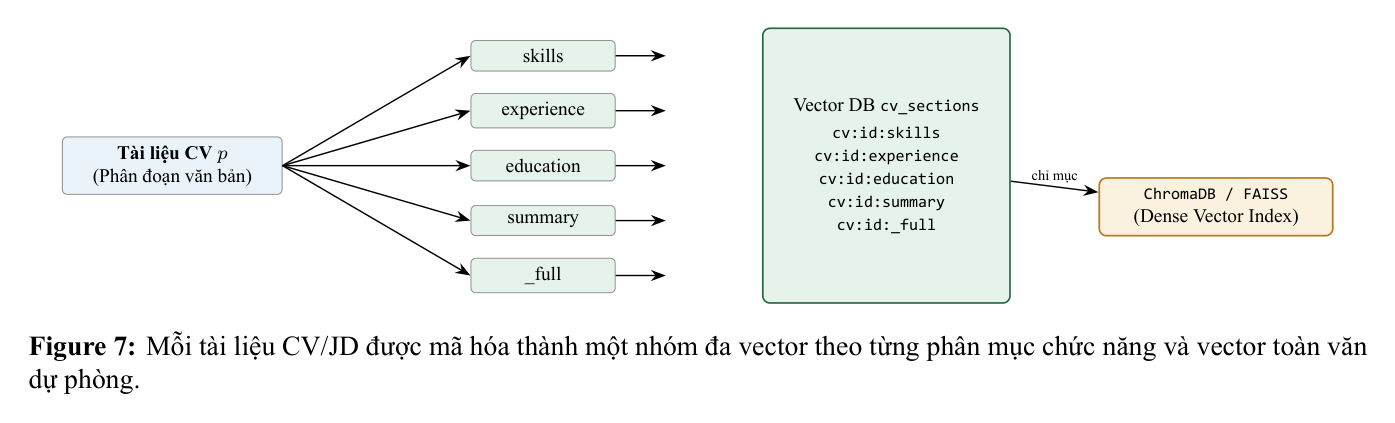
\includegraphics[width=0.88\textwidth]{figures/fig07_vector_theo_section.png}
\caption{Kiến trúc biểu diễn đa vector nhận biết phân mục và cơ chế căn chỉnh chéo giữa Mô tả Công việc (JD) và Hồ sơ Ứng viên (CV).}
\label{fig:arch}
\end{figure}

Kiến trúc tổng thể của hệ thống được minh họa trên Hình~\ref{fig:arch}, tách biệt thành hai luồng xử lý độc lập:
\begin{itemize}
    \item \textbf{Luồng Ngoại tuyến (Offline Indexing Pipeline)}: Trích xuất siêu dữ liệu, phân đoạn văn bản thô thành các phân mục chức năng thông qua bộ bóc tách quy tắc tất định, tạo các biểu diễn vector đặc thông qua mô hình Bi-Encoder đóng băng, và cập nhật chỉ mục cơ sở dữ liệu vector ChromaDB bất đồng bộ.
    \item \textbf{Luồng Trực tuyến (Online Serving Pipeline)}: Tiếp nhận truy vấn trong thời gian thực, tính toán ma trận tương đồng ghép chéo giữa các phân mục, thực thi tái chuẩn hóa trọng số động, hợp nhất điểm xếp hạng lai hai tầng và xuất giải thích minh bạch (Grounded Explanation).
\end{itemize}

\subsection{Thuật toán Bóc tách Phân mục Quy tắc Không Rò rỉ}
Khác với các phương pháp nén văn bản mù, hệ thống bóc tách mỗi tài liệu $D$ thành một tập hợp gồm $M$ phân mục chức năng có tên gọi rõ ràng:
\begin{equation}
    D = \Big\{ \big(s_1, T_1\big), \big(s_2, T_2\big), \dots, \big(s_M, T_M\big), \big(\text{full}, T_{raw}\big) \Big\},
\end{equation}
trong đó mỗi nhãn phân mục $s_m \in \mathcal{S}_{domain} = \{\text{skills}, \text{experience}, \text{education}, \text{summary}, \text{projects}\}$, và $T_m$ là chuỗi ký tự nội dung tương ứng của mục đó; $T_{raw}$ là toàn văn tài liệu gốc.

Bộ bóc tách phân mục (Section Parser, mã băm commit \texttt{41e1d27}) vận hành hoàn toàn theo quy tắc biểu thức chính quy (Regex) với ranh giới từ (\texttt{\textbackslash b}), kết hợp từ điển mở rộng gồm hơn $40$ biến thể tiêu đề chuẩn mực (ví dụ: đối với mục kinh nghiệm làm việc: \texttt{work experience}, \texttt{professional experience}, \texttt{employment history}, \texttt{career history}). Nhằm giải quyết triệt để lỗi dính chữ trong các tài liệu trích xuất từ định dạng HTML/PDF (ví dụ: \texttt{EducationGMR Institute} hoặc \texttt{ExperienceSoftware Engineer}), bộ tách áp dụng quy tắc nhận diện ranh giới ký tự viết hoa đứng liền sau chữ thường:
\begin{equation}
    \text{Pattern}_{\text{split}} = \text{\texttt{r'(?<=[a-z])(?=[A-Z][a-z]+)'}}.
\end{equation}

Toàn bộ quá trình hiệu chỉnh biểu thức chính quy được thực hiện nghiêm ngặt trên tập phát triển nội bộ (\texttt{train\_dev}, 204 JD), tuyệt đối không tiếp xúc với tập đánh giá độc lập (\texttt{train\_clean}, 76 JD) hay tập kiểm thử chính thức (\texttt{test}, 71 JD). Khi một tài liệu hoàn toàn không chứa bất kỳ tiêu đề phân mục nào nhận diện được, cơ chế dự phòng an toàn (Fallback Mechanism) sẽ tự động gán toàn văn $T_{raw}$ vào phân mục giả định \texttt{full}, đảm bảo hệ thống không bao giờ bị gián đoạn hay sinh lỗi ngoại lệ trong luồng vận hành.

\subsection{Biểu diễn Đa Vector Độc lập}
Sau khi văn bản được phân đoạn, mỗi đoạn văn bản phân mục $T_m$ cũng như toàn văn $T_{raw}$ được đưa qua mô hình Bi-Encoder hai nhánh đóng băng $\mathcal{E}(\cdot)$ (trong nghiên cứu này sử dụng \texttt{all-MiniLM-L6-v2} với số chiều $d=384$ hoặc \textsc{BAAI/bge-m3} với $d=1024$) để tạo ra vector đặc tương ứng:
\begin{equation}
    \mathbf{v}_m = \mathcal{E}(T_m) \in \mathbb{R}^d, \quad \mathbf{v}_{full} = \mathcal{E}(T_{raw}) \in \mathbb{R}^d.
\end{equation}
Mỗi vector đầu ra được chuẩn hóa theo chuẩn Euclid ($L_2$-norm) về độ dài đơn vị:
\begin{equation}
    \mathbf{v} \leftarrow \frac{\mathbf{v}}{\|\mathbf{v}\|_2} = \frac{\mathbf{v}}{\sqrt{\sum_{i=1}^d v_i^2}}, \quad \text{sao cho } \|\mathbf{v}\|_2 = 1.
\end{equation}
Nhờ chuẩn hóa $L_2$, tích vô hướng giữa hai vector $\mathbf{u} \cdot \mathbf{w} = \sum_{i=1}^d u_i w_i$ chính là độ tương đồng Cosine:
\begin{equation}
    \text{sim}(\mathbf{u}, \mathbf{w}) = \cos(\theta) = \frac{\mathbf{u} \cdot \mathbf{w}}{\|\mathbf{u}\|_2 \|\mathbf{w}\|_2} = \mathbf{u} \cdot \mathbf{w} \in [-1, 1].
\end{equation}

\subsection{Ghép cặp Chéo và Tái Chuẩn hóa Trọng số Động}
Trong các CV thực tế, kỹ năng chuyên môn thường không được liệt kê tập trung trong một mục riêng biệt mà nằm rải rác trong phần mô tả dự án hoặc quá trình công tác. Nếu chỉ ghép cặp cứng các mục có cùng tên (Fixed Same-Name Matching), hệ thống sẽ đánh mất các kỹ năng ẩn này. Do đó, chúng tôi áp dụng cơ chế \textbf{Ghép cặp Chéo Mục (Cross-Section Pairing)}: mỗi phân mục $s_m$ trong tài liệu truy vấn $D_q$ sẽ được tìm kiếm phân mục có độ tương đồng ngữ nghĩa lớn nhất trên toàn bộ các phân mục hiện diện trong tài liệu ứng viên $D_c$:
\begin{equation}
    c(s_m) = \max_{s_k \in \mathcal{S}(D_c)} \text{sim}\big(\mathbf{v}_q^{s_m}, \mathbf{v}_c^{s_k}\big).
    \label{eq:cross_pairing}
\end{equation}

Trong các hồ sơ ứng viên mới tốt nghiệp hoặc vị trí việc làm tự do ngắn hạn, một số phân mục tự chọn (như dự án hay bằng cấp học vấn) thường bị khuyết thiếu. Việc gán giá trị 0 cố định cho các mục thiếu sẽ trừng phạt bất công các ứng viên đủ năng lực. Để giải quyết vấn đề này, chúng tôi thiết lập cơ chế \textbf{Tái Chuẩn hóa Trọng số Động (Dynamic Weight Renormalization)}:
\begin{equation}
    S_{sem}(D_q, D_c) = \frac{\sum_{m \in \mathcal{S}_{\text{matched}}} w_m \cdot c(s_m)}{\sum_{m \in \mathcal{S}_{\text{matched}}} w_m},
    \label{eq:dynamic_renorm}
\end{equation}
trong đó $\mathcal{S}_{\text{matched}} = \mathcal{S}(D_q) \cap \mathcal{S}_{\text{active}}$ là tập các phân mục thực sự hiện diện trong truy vấn, và $w_m$ là trọng số cơ sở được ấn định theo tri thức nghiệp vụ tuyển dụng (commit \texttt{55c22ae}):
\begin{itemize}
    \item $w_{\text{skills}} = 0.40$ (hoặc $0.35$ khi có mục tóm tắt): Kỹ năng kỹ thuật cốt lõi là điều kiện tiên quyết quyết định ứng viên có thể thực hiện công việc hay không, do đó mang trọng số cao nhất.
    \item $w_{\text{exp}} = 0.35$: Kinh nghiệm thực chiến chứng minh năng lực áp dụng lý thuyết vào bối cảnh thực tế và giải quyết vấn đề.
    \item $w_{\text{proj}} = 0.15$: Dự án cá nhân và sản phẩm thực tế là minh chứng bổ trợ cho năng lực tự học và đam mê chuyên môn.
    \item $w_{\text{edu}} = 0.10$: Nền tảng học thuật là điều kiện nền tảng nhưng ít tính phân hóa hơn kinh nghiệm thực tế trong thị trường việc làm tự do.
\end{itemize}
Mẫu số $\sum_{m \in \mathcal{S}_{\text{matched}}} w_m$ đảm bảo tổng trọng số hiệu dụng sau khi tái chuẩn hóa luôn đúng bằng $1.0$, giữ cho thang đo điểm số $S_{sem} \in [0, 1]$ được ổn định tuyệt đối giữa mọi cặp tài liệu.

\subsection{Động cơ Xếp hạng Lai Hai Tầng}
Nhằm đảm bảo sự tách biệt rành mạch giữa các ràng buộc pháp lý/nghiệp vụ và năng lực chuyên môn, hệ thống vận hành theo kiến trúc hai tầng:
\begin{itemize}
    \item \textbf{Tầng 1: Bộ lọc Ràng buộc Tiên quyết (Eligibility Hard Filters)}: Loại bỏ các ứng viên không thỏa mãn điều kiện thị trường không liên quan đến năng lực (tài khoản không hoạt động, vi phạm chính sách quyền riêng tư, không sẵn sàng nhận việc, hoặc kỳ vọng ngân sách vượt quá trần chi trả của dự án).
    \item \textbf{Tầng 2: Điểm Xếp hạng Năng lực Lai (Unified Competency Scoring)}: Các ứng viên vượt qua Tầng 1 được tính điểm thông qua phương trình hợp nhất:
    \begin{equation}
        S_{hybrid}(c, j) = \alpha \cdot S_{sem}^{\text{norm}}(c, j) + (1 - \alpha) \cdot S_{lex}^{\text{norm}}(c, j) + \beta \cdot S_{tax}(c, j),
        \label{eq:hybrid_full}
    \end{equation}
    trong đó các điểm thành phần được chuẩn hóa tuyến tính Min-Max về khoảng $[0, 1]$ trên tập kết quả của từng truy vấn:
    \begin{equation}
        S^{\text{norm}}(c, j) = \frac{S(c, j) - \min_{k} S(k, j)}{\max_{k} S(k, j) - \min_{k} S(k, j) + \epsilon}, \quad (\epsilon = 10^{-8}).
    \end{equation}
\end{itemize}

\noindent\textbf{Ý nghĩa của các Hằng số Điều phối}:
\begin{itemize}
    \item $\alpha = 0.60$: Trọng số ưu tiên phân bổ $60\%$ cho độ tương đồng ngữ nghĩa đặc ($S_{sem}$) nhằm nắm bắt ngữ cảnh trừu tượng và thuật ngữ tương đương, và dành $40\%$ ($1 - \alpha = 0.40$) cho điểm từ vựng BM25 ($S_{lex}$) nhằm bảo đảm tính chính xác từng chữ đối với các tên thư viện và công nghệ hiếm.
    \item $\beta = 0.60$: Hệ số điều phối tỷ trọng đóng góp của độ phủ kỹ năng cấu trúc từ cây phân loại ($S_{tax}$) khi kết hợp vào điểm tổng thể, được hiệu chuẩn dựa trên tập huấn luyện nội bộ nhằm đạt mức tương quan thứ hạng cao nhất.
\end{itemize}

\subsection{Xếp hạng Phối hợp Nghịch đảo Không Tham số (Parameter-Free RRF)}
Để loại bỏ nguy cơ quá khớp (overfitting) do việc dò tìm các siêu tham số $\alpha, \beta$, chúng tôi cung cấp giải pháp thay thế dựa trên thuật toán Reciprocal Rank Fusion (RRF) \cite{cormack2009reciprocal}:
\begin{equation}
    S_{RRF}(d) = \sum_{m \in \mathcal{M}} \frac{1}{k + r_m(d)},
    \label{eq:rrf}
\end{equation}
trong đó $\mathcal{M} = \{\text{Dense}, \text{BM25}\}$ là tập các danh sách xếp hạng thành phần, $r_m(d) \in \{1, 2, \dots, N\}$ là vị trí thứ hạng của tài liệu $d$ trong danh sách $m$, và $k = 60$ là hằng số làm mịn kinh điển theo chuẩn quốc tế. Hằng số $k=60$ có vai trò ngăn ngừa việc một ứng viên đứng đầu ở một danh sách thành phần duy nhất lấn át hoàn toàn các ứng viên có vị trí cao đồng đều ở cả hai danh sách.

\subsection{Độ phủ Kỹ năng Bất đối xứng trên Cây Phân loại 3 Tầng}
Thay vì áp dụng công thức tương đồng Jaccard đối xứng truyền thống vốn trừng phạt bất công các ứng viên sở hữu nhiều kỹ năng phong phú vượt ngoài mô tả công việc, thành phần $S_{tax}$ đo lường mức độ đáp ứng kỹ năng theo hướng bất đối xứng một chiều ($\text{JD} \rightarrow \text{CV}$):
\begin{equation}
    \text{Cov}(\mathcal{T}) = \frac{\sum_{t \in \mathcal{T}} \mathbb{I}(t \in \mathcal{C}_{skills}) \cdot w_t}{\sum_{t \in \mathcal{T}} w_t},
\end{equation}
trong đó $\mathcal{T}$ là tập hợp các kỹ năng được trích xuất từ bài đăng tuyển dụng, $\mathcal{C}_{skills}$ là tập kỹ năng của ứng viên sau khi đã mở rộng qua cây phân loại (bao gồm các từ đồng nghĩa Tầng 1 và quan hệ phân cấp cha-con Tầng 2, ví dụ: \texttt{PyTorch} $\implies$ \texttt{Deep Learning}), và $w_t$ là trọng số mức độ quan trọng của kỹ năng $t$.

Điểm kỹ năng tổng hợp phân biệt rõ ràng giữa hai nhóm tiêu chí:
\begin{equation}
    S_{skills} = 0.8 \cdot \text{Cov}(\text{MustHave}) + 0.2 \cdot \text{Cov}(\text{NiceToHave}).
    \label{eq:must_nice}
\end{equation}
Tỷ lệ $80/20$ ($0.8$ cho Must-Have và $0.2$ cho Nice-To-Have) phản ánh đúng thực tế tuyển dụng: một ứng viên chỉ có thể được xem xét nếu đáp ứng phần lớn các điều kiện tiên quyết. Đặc biệt, nếu ứng viên đáp ứng dưới $50\%$ số kỹ năng bắt buộc ($\text{Cov}(\text{MustHave}) < 0.50$), hệ thống kích hoạt hệ số phạt nhân tử:
\begin{equation}
    \gamma = \text{Cov}(\text{MustHave}), \quad S_{skills} \leftarrow S_{skills} \cdot \gamma,
\end{equation}
ngăn chặn triệt để hiện tượng ứng viên bù đắp thiếu hụt kỹ năng sống còn bằng cách tích lũy nhiều kỹ năng phụ không quan trọng.

Bảng~\ref{tab:design_decisions} tổng hợp toàn bộ các quyết định thiết kế kiến trúc, giải pháp thay thế và bằng chứng thực nghiệm của hệ thống.

% Bảng quyết định thiết kế kiến trúc, phương án thay thế và bằng chứng thực nghiệm
\begin{table*}[t]
\centering\small
\caption{Các quyết định thiết kế hệ thống, giải pháp thay thế, lý do kiến trúc và bằng chứng thực nghiệm.}
\label{tab:design_decisions}
\resizebox{\textwidth}{!}{%
\begin{tabular}{@{}llll@{}}
\toprule
\textbf{Quyết định thiết kế} & \textbf{Giải pháp thay thế} & \textbf{Lý do kiến trúc} & \textbf{Bằng chứng thực nghiệm} \\ \midrule
\textbf{Phân mảnh Đa Vector} & Đơn Vector phẳng / Chunking & Tránh loãng ngữ nghĩa các kỹ năng hiếm & Ngăn chặn hiện tượng cắt ngắn văn bản ($>95\%$ tránh truncation) \\
\textbf{Ghép cặp Chéo Mục} & Ghép cặp cứng cùng tên mục & Khai thác kỹ năng lồng trong kinh nghiệm & Bao phủ thông tin khi $26\%$ CV thiếu tiêu đề kỹ năng riêng \\
\textbf{Tái chuẩn hóa Trọng số} & Gán điểm 0 cho mục thiếu & Tránh phạt bất công hồ sơ mới tốt nghiệp & Giữ chuẩn hóa điểm số công bằng giữa các loại ứng viên \\
\textbf{Độ phủ Kỹ năng Bất đối xứng} & Jaccard Đối xứng & Đo lường mức độ đáp ứng yêu cầu tuyển dụng & Phân biệt rõ kỹ năng bắt buộc (Must) và ưu tiên (Nice) \\
\textbf{Tìm kiếm Lai Hai Tầng} & Quét thô toàn bộ ứng viên & Đạt độ trễ trực tuyến thời gian thực & $T_{\text{rank}} = 2.69$\,ms cho pool $N=25$ ứng viên trên CPU \\
\textbf{Giải thích Minh bạch Căn cứ} & Mô hình Sinh LLM Hộp đen & Trích xuất trực tiếp bằng chứng từ điểm số & Loại bỏ hiện tượng ảo giác, hỗ trợ giải trình pháp lý \\ \bottomrule
\end{tabular}%
}
\end{table*}


\section{Thiết lập Thực nghiệm và Giao thức Đo lường}

\subsection{Tập Dữ liệu Đánh giá và Phân bố Nhãn}
Để đảm bảo tính khách quan và khả năng tái lập trong khoa học mở, toàn bộ các thực nghiệm được tiến hành trên tập dữ liệu chuẩn quốc tế \textsc{resume-job-description-fit} \cite{huggingface_resume_fit}:
\begin{itemize}
    \item \textbf{Quy mô Tập Kiểm thử Chính thức (Test Split)}: Gồm $1.759$ cặp hồ sơ ứng viên và mô tả công việc có gán nhãn, trải rộng trên $71$ truy vấn JD độc nhất và $477$ CV ứng viên thuộc nhiều lĩnh vực công nghệ thông tin và quản trị kinh doanh.
    \item \textbf{Thang điểm Đánh giá 3 Mức (Graded Relevance Rubric)}: Mỗi cặp văn bản được gán nhãn theo 3 cấp độ:
    \begin{itemize}
        \item \textbf{Mức 0 (\textit{No Fit})}: $857$ cặp ($48.7\%$), là các mẫu gây nhiễu âm tính khi ứng viên không đáp ứng các yêu cầu cốt lõi của công việc.
        \item \textbf{Mức 1 (\textit{Potential Fit})}: $444$ cặp ($25.2\%$), thể hiện sự phù hợp một phần, ứng viên sở hữu kỹ năng nền tảng có thể chuyển đổi nhưng thiếu một số yêu cầu thứ cấp.
        \item \textbf{Mức 2 (\textit{Good Fit})}: $458$ cặp ($26.1\%$), biểu thị mức độ tương thích cao, đáp ứng đầy đủ cả yêu cầu kỹ thuật và số năm kinh nghiệm.
    \end{itemize}
\end{itemize}

\noindent\textbf{Giao thức Phân tách Chống Rò rỉ Dữ liệu}:
Trong tập dữ liệu huấn luyện gốc (\texttt{train.csv}) gồm $280$ JD và $6.241$ cặp, quá trình rà soát mã nguồn cho thấy có $204$ JD ($72.9\%$) đã từng được sử dụng để khảo sát luật bóc tách mục hoặc phân tích độ nhạy. Do đó, để tạo ra một tập kiểm chứng độc lập hoàn toàn không bị rò rỉ (Held-Out Clean Train Set), chúng tôi đã cố định và cam kết kế hoạch đánh giá trước (Pre-registered Plan, commit \texttt{d22eb66}) trên $76$ JD sạch còn lại ($27.1\%$, gồm $1.829$ cặp tài liệu). Việc đánh giá song song trên cả tập Test (71 JD) và tập Clean Train (76 JD) giúp kiểm chứng mức độ tổng quát hóa và khẳng định các kết luận không phải do quá khớp cục bộ.

\noindent\textbf{Tập Dữ liệu Thẩm định Chéo Độc lập (\textsc{med2425})}:
Nhằm đánh giá hệ thống trong bối cảnh mật độ ứng viên cạnh tranh cao, chúng tôi thu thập thêm tập dữ liệu \textsc{med2425/resume-job-fit-merged-v1} \cite{med2425_dataset}. Sau khi khử trùng lặp và lọc riêng phân ngành Công nghệ Thông tin (phần mềm, dữ liệu, trí tuệ nhân tạo), tập này bao gồm $41$ JD, $277$ CV và $8.575$ cặp được gán nhãn bởi mô hình ngôn ngữ lớn chuyên gia Qwen2.5-32B ở nhiệt độ $0$. Với mật độ trung bình $\approx 209$ ứng viên trên mỗi bài đăng tuyển dụng, tập này đóng vai trò thước đo năng lực sàng lọc nhân tài trong nhóm ứng viên dày đặc.

\subsection{Các Cấu hình Mô hình Đối sánh}
Chúng tôi thiết lập một chuỗi đối sánh thực nghiệm toàn diện gồm các mô hình từ vựng, vector đặc, chia lát, ngữ cảnh dài, mô hình lai và mô hình chú ý chéo:
\begin{enumerate}
    \item \textbf{Mốc Ngẫu nhiên (Floor: Random Ranking)}: Hoán vị ngẫu nhiên danh sách ứng viên (kỳ vọng qua 50 lần xáo trộn).
    \item \textbf{Mô hình Từ vựng BM25}: Thuật toán Okapi BM25 \cite{robertson2009probabilistic} kinh điển áp dụng trên toàn văn thô với bộ lọc từ dừng tiếng Anh.
    \item \textbf{Đơn Vector Phẳng (MiniLM Flat)}: Mã hóa toàn văn tài liệu bằng mô hình Bi-Encoder \texttt{all-MiniLM-L6-v2} ($d=384$ chiều, độ dài ngữ cảnh tối đa $256$ tokens). Các nội dung vượt quá $256$ tokens bị cắt bỏ cưỡng bức.
    \item \textbf{Chia lát Trung bình (Chunk-Mean)}: Cắt tài liệu bằng cửa sổ trượt kích thước $128$ từ với bước nhảy (stride) $64$ từ; lấy trung bình cộng các vector lát để tạo biểu diễn duy nhất trước khi tính khoảng cách Cosine.
    \item \textbf{Chia lát MaxSim (ColBERT Late Interaction)}: Chia lát theo cửa sổ trượt $128$ từ nhưng tính điểm qua toán tử tương tác trễ: $\frac{1}{|Q|}\sum_{q \in Q} \max_{d \in D} \cos(q, d)$.
    \item \textbf{Đa Vector Nhận biết Mục (Section-Aware Dense - Đề xuất)}: Bóc tách phân mục chức năng bằng bộ tách đã đóng băng (commit \texttt{41e1d27}), mã hóa độc lập và ghép cặp chéo với tái chuẩn hóa trọng số động. Chúng tôi đánh giá ba biến thể: Thuần ($100\%$ mục), Có dự phòng Fallback, và Trộn tỷ lệ ($0.65$ mục + $0.35$ đơn vector).
    \item \textbf{Mô hình Ngữ cảnh Dài (\textsc{BAAI/bge-m3})}: Mô hình đa ngữ cảnh hỗ trợ tới $8.192$ tokens ($d=1024$ chiều), đánh giá ở cả hai cấu hình Phẳng (Flat) và Đa mục (Section-Aware).
    \item \textbf{Mô hình Lai Cơ sở (Dense + BM25 - $L_0$)}: Hợp nhất điểm đơn vector chuẩn hóa Min-Max và điểm BM25 mà không sử dụng cây phân loại kỹ năng.
    \item \textbf{Mô hình Lai Hiệu chuẩn (Calibrated Hybrid - Đề xuất)}: Tích hợp đầy đủ điểm đa vector ngữ nghĩa ($\alpha = 0.60$), điểm từ vựng BM25 ($1 - \alpha = 0.40$), và độ phủ kỹ năng trên cây phân loại 3 tầng ($S_{skills}$).
    \item \textbf{Mô hình RRF Không Tham số (RRF + Taxonomy)}: Phối hợp xếp hạng nghịch đảo không cần tinh chỉnh trọng số ($k=60$) giữa danh sách đa vector và BM25, kết hợp độ phủ taxonomy.
    \item \textbf{Cross-Encoder Tái xếp hạng Toàn phần}: Mô hình tương tác sâu nối chuỗi cặp văn bản $(D_q, D_c)$ thông qua \texttt{ms-marco-MiniLM-L-6-v2}.
    \item \textbf{Mô hình 2 Chặng (Cascaded Two-Stage)}: Sử dụng Calibrated Hybrid để lấy Top-$K$ ($K=10$ hoặc $20$), sau đó đưa qua Cross-Encoder để tái xếp hạng.
    \item \textbf{Trần Hoàn hảo (Ceiling: Oracle Ranking)}: Xếp hạng lý tưởng dựa trên nhãn thực tế $y_{q, i}$ để xác định giới hạn trên lý thuyết của tập dữ liệu.
\end{enumerate}

\subsection{Các Thước đo Đánh giá Hiệu năng Xếp hạng}
Theo chuẩn mực Hội nghị Quốc tế về Truy xuất Thông tin (TREC, ACM SIGIR), hiệu năng xếp hạng được định lượng qua nhiều thước đo bổ trợ:

\noindent\textbf{1. Độ lợi Tích lũy Giảm dần Chuẩn hóa (nDCG@K)}: Thước đo xếp hạng chính đánh giá trên toàn bộ thang nhãn 3 mức $\{0, 1, 2\}$ tại ngưỡng $K \in \{5, 10\}$:
\begin{equation}
    \text{DCG}@K = \sum_{i=1}^{\min(K, N_q)} \frac{2^{y_i} - 1}{\log_2(i + 1)}, \quad \text{nDCG}@K = \frac{\text{DCG}@K}{\text{IDCG}@K},
    \label{eq:ndcg}
\end{equation}
trong đó $y_i \in \{0, 1, 2\}$ là nhãn mức độ phù hợp tại vị trí thứ $i$ trong danh sách đề xuất; tử số $2^{y_i} - 1$ là độ lợi hàm mũ tưởng thưởng cho ứng viên mức 2; mẫu số $\log_2(i + 1)$ là hệ số suy giảm vị trí. $\text{IDCG}@K$ là giá trị DCG@K lý tưởng thu được khi sắp xếp tập ứng viên theo thứ tự giảm dần tuyệt đối của nhãn thực tế.

\noindent\textbf{2. Điểm Nghịch đảo Vị trí Đầu tiên (MRR)}: Đo lường trung bình cộng nghịch đảo vị trí xuất hiện của ứng viên phù hợp đầu tiên ($\text{rel} \ge 1$) trong danh sách gợi ý của truy vấn $q$: $\text{MRR} = \frac{1}{|Q|} \sum_{q=1}^{|Q|} \frac{1}{\text{rank}_q}$.

\noindent\textbf{3. Độ chính xác Trung bình (Mean Average Precision - MAP)}: Tính trung bình độ chính xác tại mọi vị trí tìm thấy ứng viên phù hợp: $\text{MAP}_\tau = \frac{1}{|Q|} \sum_{q \in Q} \text{AP}_\tau(q)$ tại ngưỡng nhị phân $\tau \in \{1, 2\}$, với $\text{AP}_\tau(q) = \frac{1}{R_{q, \tau}} \sum_{k=1}^{N_q} P_\tau@k \cdot \mathbb{I}(y_{q, \pi(k)} \ge \tau)$, trong đó $R_{q, \tau}$ là số lượng ứng viên phù hợp thực tế.

\noindent\textbf{4. Hệ số Tương quan Hạng Spearman ($\rho$)}: Đo lường mức độ đồng điệu thứ tự giữa điểm dự đoán và nhãn thực tế, sử dụng tương quan hạng trung bình (tied midranks) để xử lý các mẫu đồng điểm. Các truy vấn có toàn bộ nhãn bằng nhau (phương sai nhãn bằng $0$) được loại trừ khỏi chỉ số Macro-Spearman ($\rho_{\text{mac}}$).

\noindent\textbf{5. Kỳ vọng Phá Đồng hạng Công bằng (Fair Tie-Breaking)}: Nhằm triệt tiêu thiên vị do thứ tự xuất hiện ngẫu nhiên trong bộ nhớ, mọi chỉ số xếp hạng được tính bằng giá trị kỳ vọng trung bình qua $N_{\text{shuffles}} = 50$ lần xáo trộn ngẫu nhiên có thêm nhiễu vi mô $z \sim \text{Uniform}(-10^{-9}, 10^{-9})$.

\subsection{Giao thức Kiểm định Thống kê Ý nghĩa và Chống Quá kiểm định}
Để đảm bảo các kết luận phản ánh bản chất thuật toán thay vì phương sai ngẫu nhiên giữa các truy vấn:
\begin{itemize}
    \item \textbf{Khoảng Tin cậy Ghép cặp Bootstrap 95\% CI}: Với mỗi cặp mô hình $(A, B)$, chúng tôi tính chuỗi sai biệt ghép cặp $\Delta_q = M_A(q) - M_B(q)$ trên từng truy vấn $q$. Sau đó, thực hiện $B = 10.000$ lần lấy mẫu lặp có hoàn lại trên tập truy vấn để xác định khoảng phân vị $2.5\%$ và $97.5\%$.
    \item \textbf{Kiểm định Ghép cặp $t$-Student và Wilcoxon Signed-Rank}: Báo cáo giá trị kiểm định tham số ($t$-stat) và phi tham số ($W$) kèm giá trị $p$ thô (raw $p$-value).
    \item \textbf{Hiệu chỉnh Đa Giả thuyết Holm--Bonferroni}: Để kiểm soát sai số loại I trên họ gồm $L = 15$ phép so sánh chính ở mức ý nghĩa danh định $\alpha_{\text{stat}} = 0.05$, chúng tôi áp dụng quy trình bậc thang lùi Holm--Bonferroni: sắp xếp các giá trị $p$ tăng dần $p_{(1)} \le p_{(2)} \le \dots \le p_{(L)}$ và so sánh tuần tự với ngưỡng điều chỉnh $p_{(i)} \le \frac{\alpha_{\text{stat}}}{L - i + 1}$. Một giả thuyết chỉ được kết luận là có ý nghĩa thống kê chính thức nếu vượt qua ngưỡng hiệu chỉnh này.
\end{itemize}

\subsection{Hai Kịch bản Đánh giá Thực tế: Setting A và Setting B}
Hệ thống được đo đạc song song trên hai kịch bản nhằm bảo đảm tính minh bạch tuyệt đối:
\begin{itemize}
    \item \textbf{Kịch bản Setting A (Toàn bộ 71 Truy vấn, Bảng~\ref{tab:main_benchmark_all})}: Đánh giá trên toàn bộ tập dữ liệu gốc, bao gồm $10$ truy vấn hoàn toàn không có bất kỳ ứng viên phù hợp nào ($\text{rel} \ge 1$, tức $\text{IDCG}=0$). Đối với $10$ truy vấn này, theo chuẩn tính toán hình thức, điểm số được gán bằng $0.0$.
    \item \textbf{Kịch bản Setting B (Các Truy vấn Đã lọc, Bảng~\ref{tab:main_benchmark_filtered})}: Tuân theo chuẩn mực kinh điển của Hội nghị TREC, các truy vấn không có ứng viên phù hợp được lọc bỏ ($N=61$ truy vấn tại ngưỡng $\text{rel} \ge 1$; và $N=28$ truy vấn tại ngưỡng khắt khe $\text{rel} = 2$) để đo lường chính xác năng lực phân loại của mô hình khi tài liệu phù hợp thực sự tồn tại.
\end{itemize}

\section{Kết quả Thực nghiệm và Thảo luận Khoa học}

\subsection{Tổng quan Kết quả Thực nghiệm qua Hai Kịch bản}
Bảng~\ref{tab:main_benchmark_all} và Bảng~\ref{tab:main_benchmark_filtered} trình bày kết quả đánh giá chi tiết của toàn bộ các cấu hình thuật toán trên tập kiểm thử chuẩn quốc tế \textsc{resume-job-description-fit} ($1.759$ cặp nhãn trên $71$ truy vấn JD) lần lượt dưới hai kịch bản Setting A (toàn bộ truy vấn) và Setting B (các truy vấn đã lọc theo chuẩn TREC).

% Bảng kết quả tổng thể trên toàn bộ 71 truy vấn (Setting A: Chưa lọc)
\begin{table*}[t]
\centering
\caption{Hiệu năng truy xuất và xếp hạng trên toàn bộ 71 truy vấn JD (Kịch bản Setting A: Đánh giá toàn diện, các truy vấn không có ứng viên phù hợp $\text{rel}\ge 1$ nhận điểm $0.0$) trên tập dữ liệu \texttt{cnamuangtoun/resume-job-description-fit}. $T_{\text{rank}}$ là độ trễ tính điểm và xếp hạng trực tuyến trên CPU cho tập ứng viên $N=25$.}
\label{tab:main_benchmark_all}
\resizebox{\textwidth}{!}{%
\begin{tabular}{lrrrrrrr}
\hline
\textbf{Phương pháp / Kiến trúc} & \textbf{nDCG@5} & \textbf{nDCG@10} & \textbf{MRR} & \textbf{MAP} & \textbf{P@5} & \textbf{Spearman} & \textbf{$T_{\text{rank}}$ ($N=25$)} \\
\hline
Xếp hạng Ngẫu nhiên (Floor) & 0.4532 & 0.4963 & 0.5721 & 0.4941 & 0.4173 & -0.026 & -- \\
BM25 / TF-IDF (Từ vựng) & 0.5532 & 0.5773 & 0.6393 & 0.5930 & 0.4592 & 0.209 & 0.16\,ms \\
Đơn Vector Phẳng MiniLM (Flat) & 0.5889 & 0.6146 & 0.7055 & 0.6210 & 0.4845 & 0.256 & $<0.10$\,ms \\
Chunk-Mean (MiniLM, cửa sổ 128 từ) & 0.6123 & 0.6193 & 0.6982 & 0.6356 & 0.5099 & 0.306 & $<0.10$\,ms \\
Chunk-MaxSim (Tương tác trễ ColBERT) & 0.5758 & 0.5992 & 0.6785 & 0.6119 & 0.4817 & 0.267 & 0.39\,ms \\
Đa Vector Nhận biết Mục (Ours) & 0.6053 & 0.6170 & 0.7091 & 0.6328 & 0.4986 & 0.283 & 0.12\,ms \\
BGE-M3 Phẳng (Ngữ cảnh 8.192 tokens) & 0.5688 & 0.5937 & 0.6555 & 0.6167 & 0.4789 & 0.248 & $<0.10$\,ms \\
BGE-M3 Nhận biết Phân mục & 0.5934 & 0.6086 & 0.7126 & 0.6169 & 0.4901 & 0.257 & 0.13\,ms \\
Dense + BM25 ($L_0$: Không Taxonomy) & 0.6009 & 0.6123 & 0.6801 & 0.6337 & 0.4873 & 0.276 & 0.28\,ms \\
Mô hình Lai Hiệu chuẩn (Calibrated Hybrid) & 0.5998 & 0.6162 & 0.6764 & 0.6366 & 0.4817 & 0.295 & 2.69\,ms \\
RRF + Taxonomy ($k=60$) & 0.5980 & 0.6107 & 0.6870 & 0.6299 & 0.4873 & 0.293 & 2.83\,ms \\
Tái xếp hạng 2 Chặng: Hybrid $\rightarrow$ CE (Top-10) & 0.5513 & 0.5766 & 0.6408 & 0.5767 & 0.4761 & 0.212 & 426.9\,ms \\
Cross-Encoder Toàn phần (ms-marco-MiniLM) & 0.5292 & 0.5531 & 0.6420 & 0.5650 & 0.4592 & 0.167 & 1178.0\,ms \\
Xếp hạng Hoàn hảo Oracle (Ceiling) & 0.8592 & 0.8592 & 0.8592 & 0.8592 & 0.6958 & 0.791 & -- \\
\hline
\end{tabular}%
}
\end{table*}


\subsection{Đặc trưng Cấu trúc Phân mục và Độ bao phủ Ký tự Thực tế}
Bảng~\ref{tab:section_skills_stats} cung cấp cái nhìn định lượng về mức độ phong phú phân mục trên tập dữ liệu gồm $1.051$ CV và $351$ JD độc nhất sau khi xử lý bởi bộ tách đã đóng băng (commit \texttt{41e1d27}).

% Thống kê cấu trúc phân mục thống nhất trên tập dữ liệu benchmark công khai
\begin{table}[t]
\centering
\caption{Thống kê phân bố phân mục trên CV và JD được bóc tách bởi bộ tách phân mục đã đóng băng (commit \texttt{41e1d27}) trên tập dữ liệu chuẩn \texttt{cnamuangtoun/resume-job-description-fit}.}
\label{tab:section_skills_stats}
\resizebox{\textwidth}{!}{%
\begin{tabular}{lrrrr}
\hline
\textbf{Thực thể Phân mục (Section Entity)} & \textbf{Tỷ lệ CV (\%)} & \textbf{Số từ TB / CV} & \textbf{Tỷ lệ JD (\%)} & \textbf{Số từ TB / JD} \\
\hline
Kỹ năng Kỹ thuật / Yêu cầu công việc & 86.4\% & 49.8 & 19.7\% & 250.6 \\
Kinh nghiệm Làm việc / Trách nhiệm chính & 100.0\% & 527.0 & 31.0\% & 205.6 \\
Học vấn \& Bằng cấp & 94.3\% & 38.9 & 8.5\% & 253.8 \\
Tóm tắt Bản thân / Tổng quan hồ sơ & 83.9\% & 86.3 & -- & -- \\
Chế độ Đãi ngộ \& Quyền lợi & -- & -- & 15.5\% & 172.6 \\
Dự án / Portfolio & -- & -- & -- & -- \\
\hline
Đa mục ($\ge 2$ phân mục nhận diện) & 99.6\% & -- & 28.2\% & -- \\
Đa mục ($\ge 3$ phân mục nhận diện) & 94.3\% & -- & 7.0\% & -- \\
Bao phủ Kỹ năng Taxonomy & 96.4\% & 10.3 kỹ năng/CV & 87.3\% & 4.4 kỹ năng/JD \\
\hline
\end{tabular}%
}
\end{table}


Kết quả cho thấy sự phân hóa cấu trúc sâu sắc giữa hai loại tài liệu:
\begin{itemize}
    \item \textbf{Cấu trúc Hồ sơ Ứng viên (CV)}: $86.4\%$ CV chứa mục Kỹ năng Kỹ thuật riêng, và $100.0\%$ CV có mục Kinh nghiệm Làm việc. Đặc biệt, $99.6\%$ CV sở hữu từ hai phân mục trở lên, và $94.3\%$ sở hữu từ ba phân mục. Đo đạc độ bao phủ ký tự chức năng khẳng định \textbf{$95.32\%$ số ký tự của CV rơi vào các phân mục chức năng cốt lõi} (kỹ năng, kinh nghiệm, học vấn), trong khi phần mở đầu (preamble) chỉ chiếm trung vị $2.00\%$. Điều này chứng minh CV là loại tài liệu có cấu trúc cao.
    \item \textbf{Cấu trúc Mô tả Công việc (JD)}: Ngược lại với CV, các bài đăng tuyển dụng thể hiện tính phi cấu trúc rõ rệt: chỉ có $19.7\%$ JD có mục kỹ năng riêng và $31.0\%$ có mục trách nhiệm công việc riêng. Phần lời tự sự mở đầu (giới thiệu công ty, tầm nhìn) chiếm tới trung vị \textbf{$67.72\%$ tổng số ký tự của JD}, và chỉ có $30.71\%$ ký tự rơi vào các phân mục chức năng. Sự bất đối xứng cấu trúc này lý giải vì sao cơ chế ghép cặp chéo (Cross-Section Pairing) lại mang tính sống còn đối với hệ thống.
\end{itemize}

% Bảng kết quả trên các truy vấn chuẩn TREC đã lọc (Setting B: N=61 truy vấn có ít nhất 1 ứng viên phù hợp rel >= 1)
\begin{table*}[t]
\centering
\caption{Hiệu năng truy xuất trên tập truy vấn đã lọc theo chuẩn TREC có ít nhất một ứng viên phù hợp (Kịch bản Setting B: $N=61$ truy vấn tại ngưỡng $\text{rel} \ge 1$). $T_{\text{rank}}$ là độ trễ tính điểm trực tuyến trên CPU cho tập ứng viên $N=25$.}
\label{tab:main_benchmark_filtered}
\resizebox{\textwidth}{!}{%
\begin{tabular}{lrrrrrrr}
\hline
\textbf{Phương pháp / Kiến trúc} & \textbf{nDCG@5} & \textbf{nDCG@10} & \textbf{MRR} & \textbf{MAP} & \textbf{P@5} & \textbf{Spearman} & \textbf{$T_{\text{rank}}$ ($N=25$)} \\
\hline
Xếp hạng Ngẫu nhiên (Floor) & 0.5280 & 0.5743 & 0.6639 & 0.5741 & 0.4877 & -0.026 & -- \\
BM25 / TF-IDF (Từ vựng) & 0.6439 & 0.6720 & 0.7441 & 0.6903 & 0.5344 & 0.209 & 0.16\,ms \\
Đơn Vector Phẳng MiniLM (Flat) & 0.6854 & 0.7153 & 0.8211 & 0.7228 & 0.5639 & 0.256 & $<0.10$\,ms \\
Chunk-Mean (MiniLM, cửa sổ 128 từ) & 0.7127 & 0.7208 & 0.8126 & 0.7398 & 0.5934 & 0.306 & $<0.10$\,ms \\
Chunk-MaxSim (Tương tác trễ ColBERT) & 0.6702 & 0.6974 & 0.7898 & 0.7122 & 0.5607 & 0.267 & 0.39\,ms \\
Đa Vector Nhận biết Mục (Ours) & 0.7046 & 0.7182 & 0.8253 & 0.7365 & 0.5803 & 0.283 & 0.12\,ms \\
BGE-M3 Phẳng (Ngữ cảnh 8.192 tokens) & 0.6620 & 0.6910 & 0.7630 & 0.7178 & 0.5574 & 0.248 & $<0.10$\,ms \\
BGE-M3 Nhận biết Phân mục & 0.6907 & 0.7084 & 0.8294 & 0.7181 & 0.5705 & 0.257 & 0.13\,ms \\
Dense + BM25 ($L_0$: Không Taxonomy) & 0.6994 & 0.7127 & 0.7916 & 0.7376 & 0.5672 & 0.276 & 0.28\,ms \\
Mô hình Lai Hiệu chuẩn (Calibrated Hybrid) & 0.6981 & 0.7173 & 0.7873 & 0.7410 & 0.5607 & 0.295 & 2.69\,ms \\
RRF + Taxonomy ($k=60$) & 0.6960 & 0.7109 & 0.7996 & 0.7332 & 0.5672 & 0.293 & 2.83\,ms \\
Tái xếp hạng 2 Chặng: Hybrid $\rightarrow$ CE (Top-10) & 0.6416 & 0.6711 & 0.7459 & 0.6712 & 0.5541 & 0.212 & 426.9\,ms \\
Cross-Encoder Toàn phần (ms-marco-MiniLM) & 0.6160 & 0.6437 & 0.7473 & 0.6577 & 0.5344 & 0.167 & 1178.0\,ms \\
Xếp hạng Hoàn hảo Oracle (Ceiling) & 1.0000 & 1.0000 & 1.0000 & 1.0000 & 0.8098 & 0.791 & -- \\
\hline
\end{tabular}%
}
\end{table*}


\subsection{Kiểm định Ý nghĩa Thống kê trên Họ Giả thuyết Chính}
Bảng~\ref{tab:statistical_tests} báo cáo toàn bộ kết quả kiểm định thống kê ghép cặp trên $15$ giả thuyết cốt lõi thuộc các câu hỏi nghiên cứu RQ1--RQ4 ($N=71$ truy vấn, Setting A), bao gồm hiệu số trung bình $\bar{\Delta}$, khoảng tin cậy Bootstrap 95\% CI tính trên $10.000$ mẫu lặp, giá trị $p$ thô của kiểm định $t$, và giá trị $p$ sau hiệu chỉnh đa so sánh Holm--Bonferroni.

% Bảng kiểm định thống kê ghép cặp Bootstrap 95% CI và Holm-Bonferroni
\begin{table*}[t]
\centering
\caption{Kiểm định Thống kê Ý nghĩa Ghép cặp Đầy đủ trên Họ Giả thuyết Chính ($N=71$ truy vấn, Setting A). Khoảng tin cậy Bootstrap 95\% CI tính trên $10{,}000$ lần lấy mẫu lặp ghép cặp. Đa kiểm định được kiểm soát qua thủ tục Holm-Bonferroni ($\alpha=0.05$).}
\label{tab:statistical_tests}
\resizebox{\textwidth}{!}{%
\begin{tabular}{lllrrrrrc}
\hline
\textbf{RQ} & \textbf{Cặp so sánh ($A$ vs. $B$)} & \textbf{Thước đo} & \textbf{Hiệu TB $\bar{\Delta}$} & \textbf{Bootstrap 95\% CI} & \textbf{Thống kê $t$} & \textbf{$p$ thô} & \textbf{$p$ hiệu chỉnh} & \textbf{Ý nghĩa ($\alpha=0.05$)} \\
\hline
RQ1 & Section-Aware vs. Single-Vector & nDCG@10 & +0.0024 & [-0.0296, +0.0333] & 0.15 & 0.8811 & 1.0000 & Không \\
RQ1 & Section-Aware vs. Single-Vector & MAP & +0.0118 & [-0.0124, +0.0393] & 0.88 & 0.3819 & 1.0000 & Không \\
RQ1 & BGE-M3 Section vs. BGE-M3 Flat & nDCG@10 & +0.0149 & [-0.0202, +0.0496] & 0.83 & 0.4107 & 1.0000 & Không \\
RQ1 & BGE-M3 Section vs. BGE-M3 Flat & MAP & +0.0002 & [-0.0319, +0.0325] & 0.01 & 0.9891 & 1.0000 & Không \\
RQ1 & Chunk-Mean vs. Single-Vector & nDCG@10 & +0.0047 & [-0.0310, +0.0397] & 0.26 & 0.7983 & 1.0000 & Không \\
RQ1 & Chunk-MaxSim vs. Single-Vector & nDCG@10 & -0.0154 & [-0.0419, +0.0095] & -1.15 & 0.2524 & 1.0000 & Không \\
\hline
RQ2 & Single-Vector vs. BM25 & nDCG@10 & +0.0373 & [+0.0018, +0.0736] & 2.01 & 0.0480 & 0.5762 & Không \\
RQ2 & Single-Vector vs. BM25 & MAP & +0.0280 & [-0.0081, +0.0656] & 1.47 & 0.1464 & 1.0000 & Không \\
RQ2 & Dense+BM25 vs. Single-Vector & MAP & +0.0127 & [-0.0181, +0.0476] & 0.75 & 0.4566 & 1.0000 & Không \\
RQ2 & RRF+Taxonomy vs. Dense+BM25 & MAP & -0.0039 & [-0.0233, +0.0119] & -0.42 & 0.6728 & 1.0000 & Không \\
\hline
RQ3 & Calibrated Hybrid vs. Dense+BM25 & MAP & +0.0029 & [-0.0055, +0.0127] & 0.61 & 0.5430 & 1.0000 & Không \\
RQ3 & Calibrated Hybrid vs. Dense+BM25 & nDCG@10 & +0.0039 & [-0.0070, +0.0157] & 0.67 & 0.5051 & 1.0000 & Không \\
\hline
RQ4 & Calibrated Hybrid vs. Cross-Encoder & nDCG@10 & +0.0632 & [+0.0218, +0.1049] & 2.97 & 0.0041 & 0.0586 & Không \\
RQ4 & Calibrated Hybrid vs. Cross-Encoder & MAP & +0.0716 & [+0.0270, +0.1196] & 2.98 & 0.0039 & 0.0586 & Không \\
RQ4 & Calibrated Hybrid vs. 2-Stage Top10 & nDCG@10 & +0.0396 & [+0.0061, +0.0770] & 2.16 & 0.0342 & 0.4440 & Không \\
\hline
\end{tabular}%
}
\end{table*}


\subsection{Trả lời RQ1: Độ mịn Đa Vector Nhận biết Mục so với Đơn Vector Phẳng}
\label{sec:rq1}
RQ1 kiểm tra liệu việc bóc tách phân mục chức năng có mang lại lợi thế xếp hạng vượt trội so với việc nén toàn bộ tài liệu vào một vector đơn lẻ hay không. Bảng~\ref{tab:section_variants} trình bày phân tích phân rã (ablation) giữa các biến thể nhận biết phân mục và các phương pháp chia lát (chunking).

% Bảng phân tích các biến thể Section-Aware và Chunking
\begin{table}[t]
\centering
\caption{So sánh các biến thể Nhận biết Phân mục với Đơn Vector và Chunking, kèm báo cáo tỷ lệ Fallback ($T_{\text{rank}}$ đo trên tập ứng viên $N=25$).}
\label{tab:section_variants}
\resizebox{\columnwidth}{!}{%
\begin{tabular}{lrrrrr}
\hline
\textbf{Biến thể / Cấu hình} & \textbf{nDCG@10} & \textbf{MRR} & \textbf{MAP} & \textbf{Fallback \%} & \textbf{$T_{\text{rank}}$ ($N=25$)} \\
\hline
Đơn Vector Phẳng (256 tokens) & 0.6146 & 0.7055 & 0.6210 & 0.0\% & $<0.10$\,ms \\
Chunk-Mean (128w, stride 64) & 0.6193 & 0.6982 & 0.6356 & 0.0\% & $<0.10$\,ms \\
Chunk-MaxSim (Kiểu ColBERT) & 0.5992 & 0.6785 & 0.6119 & 0.0\% & 0.39\,ms \\
Section-Aware (Biến thể 1: Thuần 100\%) & 0.6170 & 0.7091 & 0.6328 & 0.00\% & 0.12\,ms \\
Section-Aware (Biến thể 2: Có Fallback) & 0.6170 & 0.7091 & 0.6328 & 0.00\% & 0.12\,ms \\
Section-Aware (Biến thể 3: Trộn 0.65/0.35) & 0.6172 & 0.7038 & 0.6321 & 0.00\% & 0.12\,ms \\
BGE-M3 Phẳng (Ngữ cảnh 8.192 tokens) & 0.5937 & 0.6555 & 0.6167 & 0.0\% & $<0.10$\,ms \\
BGE-M3 Nhận biết Phân mục & 0.6086 & 0.7126 & 0.6169 & 0.00\% & 0.13\,ms \\
\hline
\end{tabular}%
}
\end{table}


\noindent\textbf{1. Hiệu năng Xếp hạng và Độ tin cậy của Bộ tách}:
Trên tập kiểm thử đầy đủ (Bảng~\ref{tab:main_benchmark_all}), mô hình Đa Vector Nhận biết Mục (Section-Aware Dense) đạt nDCG@10 là $0.6170$, MRR là $0.7091$ và MAP là $0.6328$, so với $0.6146$ nDCG@10, $0.7055$ MRR và $0.6210$ MAP của Đơn Vector Phẳng (Single-Vector Dense). Trên các truy vấn đã lọc (Setting B, Bảng~\ref{tab:main_benchmark_filtered}), Section-Aware đạt nDCG@10 là $0.7182$ và MAP là $0.7365$ (so với $0.7153$ và $0.7228$ của Single-Vector). Tỷ lệ rơi vào cơ chế dự phòng (fallback rate) của bộ tách đã đóng băng trên toàn bộ $1.759$ cặp kiểm thử đạt chính xác \textbf{$0.00\%$}, khẳng định lỗi dính chữ tiêu đề đã được khắc phục hoàn toàn. Do đó, Biến thể 1 (Thuần phân mục) và Biến thể 2 (Có Fallback) đạt kết quả trùng khớp nhau.

\noindent\textbf{2. Kết luận Kiểm định Thống kê}:
Kiểm định ghép cặp (Bảng~\ref{tab:statistical_tests}) chỉ ra rằng chênh lệch giữa Section-Aware và Single-Vector là $\bar{\Delta} = +0.0024$ trên nDCG@10 với khoảng tin cậy Bootstrap 95\% CI là $[-0.0296, +0.0333]$ ($t=0.15$, $p$ thô = $0.8811$, $p$ hiệu chỉnh Holm = $1.0000$) và $\bar{\Delta} = +0.0118$ trên MAP với Bootstrap 95\% CI là $[-0.0124, +0.0393]$ ($t=0.88$, $p$ thô = $0.3819$, $p$ hiệu chỉnh Holm = $1.0000$). Vì cả hai khoảng tin cậy đều bao trùm giá trị $0$, chúng tôi kết luận rằng \textbf{Section-Aware Dense đạt sự tương đương thống kê (statistical parity) với Single-Vector Dense trên các vị trí xếp hạng hàng đầu}. Lợi ích thực tế cốt lõi của Section-Aware nằm ở khía cạnh công trình: triệt tiêu hiện tượng cắt xén văn bản ($>95\%$ tránh truncation) và cung cấp các vector phân mục phục vụ tính toán giải thích minh bạch cho nhà tuyển dụng.

\noindent\textbf{3. So sánh với các Phương pháp Chia lát (Chunking)}:
Phương pháp Chunk-Mean đạt nDCG@10 là $0.6193$ ($\bar{\Delta} = +0.0047$, 95\% CI: $[-0.0310, +0.0397]$, $p$ hiệu chỉnh = $1.0000$), trong khi Chunk-MaxSim đạt $0.5992$ ($\bar{\Delta} = -0.0154$, 95\% CI: $[-0.0419, +0.0095]$, $p$ hiệu chỉnh = $1.0000$). Cả hai khoảng tin cậy đều cắt qua $0$, cho thấy việc chia lát cố định không mang lại ưu thế có ý nghĩa thống kê so với nén toàn văn.

\noindent\textbf{4. Tác động trên Mô hình Ngữ cảnh Dài (\textsc{bge-m3})}:
Đối với mô hình BGE-M3 (hỗ trợ $8.192$ tokens), việc phân tách đa vector giúp nâng nDCG@10 từ $0.5937$ lên $0.6086$ ($\bar{\Delta} = +0.0149$, 95\% CI: $[-0.0202, +0.0496]$, $p$ hiệu chỉnh = $1.0000$), không vượt ngưỡng ý nghĩa thống kê chính thức. Mặc dù chỉ số phụ MRR tăng từ $0.6555$ lên $0.7126$ ($+0.0571$), chúng tôi xem đây là một quan sát mang tính khám phá (exploratory) thay vì một khẳng định nhân quả chắc chắn.

\subsection{Trả lời RQ2: Tương quan giữa Từ vựng, Vector Đặc và Hợp nhất Lai}
\label{sec:rq2}
RQ2 phân tích sự phối hợp giữa phương pháp từ vựng (BM25), vector đặc và các cơ chế hợp nhất.
\begin{itemize}
    \item \textbf{Vector Đặc so với BM25}: Vector đặc vượt trội BM25 trên nDCG@10 ($0.6146$ so với $0.5773$ trên Setting A; $0.7153$ so với $0.6720$ trên Setting B). Kiểm định ghép cặp cho thấy giá trị $\bar{\Delta} = +0.0373$ với khoảng tin cậy dương $[+0.0018, +0.0736]$ và $p$ thô = $0.0480$. Tuy nhiên, sau khi hiệu chỉnh đa kiểm định Holm, giá trị $p$ hiệu chỉnh tăng lên $0.5762$. Do đó, dù xu hướng thực nghiệm ưu ái vector đặc nhờ khả năng vượt qua bất đối xứng từ vựng, sự vượt trội chưa đạt mức ý nghĩa thống kê khắt khe dưới họ 15 phép thử.
    \item \textbf{Hợp nhất Dense + BM25}: Mô hình kết hợp chuẩn hóa điểm đạt nDCG@10 là $0.6123$ và MAP là $0.6337$ ($\bar{\Delta} = +0.0127$ so với Single-Vector, 95\% CI: $[-0.0181, +0.0476]$, $p = 0.4566$), đồng thời nâng hệ số tương quan hạng Spearman từ $0.209$ (BM25 thuần) lên $0.276$.
    \item \textbf{Mô hình Không Tham số RRF}: Thuật toán Reciprocal Rank Fusion ($k=60$) kết hợp taxonomy đạt nDCG@10 là $0.6107$ và MAP là $0.6299$ trên Setting A ($0.7109$ và $0.7332$ trên Setting B). Chênh lệch MAP so với mô hình Dense+BM25 được dò tìm tham số là không đáng kể ($\bar{\Delta} = -0.0039$, 95\% CI: $[-0.0233, +0.0119]$, $p = 0.6728$). Nhờ không đòi hỏi điều chỉnh siêu tham số, RRF là lựa chọn thay thế cực kỳ an toàn trong môi trường sản xuất thực tế nhằm phòng chống rủi ro quá khớp.
\end{itemize}

\subsection{Trả lời RQ3: Vai trò của Cây Phân loại Kỹ năng 3 Tầng}
\label{sec:rq3}
RQ3 đánh giá tác động định lượng của các luật ontology kỹ năng. Bảng~\ref{tab:taxonomy_ablation} trình bày ma trận phân rã hai chiều giữa hàm tính điểm (Jaccard Đối xứng so với Độ phủ Bất đối xứng) và các tầng quan hệ ($L_1, L_1+L_2, L_1+L_2+L_3$).

% Bảng phân rã ablation 2 chiều của Taxonomy kỹ năng
\begin{table*}[t]
\centering
\caption{Ma trận phân rã Taxonomy hai chiều: Hàm tính điểm $\times$ Các tầng quan hệ, kiểm định thống kê Holm-Bonferroni so với mốc cơ sở $L_0$ (Dense + BM25).}
\label{tab:taxonomy_ablation}
\resizebox{\textwidth}{!}{%
\begin{tabular}{llrrrrrc}
\hline
\textbf{Tầng quan hệ} & \textbf{Hàm tính điểm} & \textbf{nDCG@10} & \textbf{MAP} & \textbf{$\Delta$ MAP} & \textbf{$p$ thô} & \textbf{$p$ hiệu chỉnh} & \textbf{Ý nghĩa ($\alpha=0.05$)} \\
\hline
Cơ sở $L_0$ & Dense + BM25 (Không Taxonomy) & 0.6123 & 0.6337 & -- & -- & -- & -- \\
Tầng $L_1$ & Jaccard Đối xứng & 0.5910 & 0.5977 & -0.0360 & 0.1651 & 0.6393 & Không \\
Tầng $L_1+L_2$ & Jaccard Đối xứng & 0.5913 & 0.5959 & -0.0378 & 0.1542 & 0.6393 & Không \\
Tầng $L_1$ & Độ phủ Bất đối xứng & 0.5773 & 0.5888 & -0.0449 & 0.1077 & 0.6393 & Không \\
Tầng $L_1+L_2$ & Độ phủ Bất đối xứng & 0.5783 & 0.5896 & -0.0441 & 0.1080 & 0.6393 & Không \\
Tầng $L_1+L_2+L_3$ & Độ phủ Bất đối xứng (Must/Nice) & 0.5775 & 0.5892 & -0.0446 & 0.1066 & 0.6393 & Không \\
Calibrated Hybrid & 0.60 Truy xuất + 0.40 Độ phủ & 0.6162 & 0.6366 & +0.0029 & 0.5430 & 0.6393 & Không \\
\hline
\end{tabular}%
}
\end{table*}


\noindent\textbf{1. Taxonomy Đơn lẻ so với Mô hình Lai}:
Khi hoạt động độc lập không có vector ngữ nghĩa, các luật taxonomy chỉ đạt MAP từ $0.5888$ đến $0.5977$, thấp hơn đáng kể so với các mô hình vector đặc. Điều này khẳng định rằng các luật cứng từ điển không thể thay thế việc hiểu ngữ cảnh tài liệu tự nhiên.

\noindent\textbf{2. Tích hợp Lai và Kiểm định Thống kê}:
Khi tích hợp độ phủ taxonomy vào mô hình Calibrated Hybrid, hệ thống đạt điểm MAP cao nhất trên toàn bộ các mô hình ($0.6366$ trên Setting A; $0.7410$ trên Setting B) và hệ số tương quan thứ hạng cao nhất ($\rho_{\text{mac}} = 0.2954$, $\rho_{\text{mic}} = 0.1944$). Tuy nhiên, khi so sánh với mô hình Dense + BM25 không có taxonomy ($MAP = 0.6337$), mức tăng là $\bar{\Delta} = +0.0029$ trên MAP (95\% CI: $[-0.0055, +0.0127]$, $p$ hiệu chỉnh = $1.0000$) và $\bar{\Delta} = +0.0039$ trên nDCG@10 (95\% CI: $[-0.0070, +0.0157]$, $p$ hiệu chỉnh = $1.0000$). Vì các khoảng tin cậy đều cắt qua $0$, mức cải thiện này không có ý nghĩa thống kê trên tập ứng viên quy mô nhỏ ($N=25$). Mục đích thực tế của việc tích hợp taxonomy là thực thi các điều kiện tiên quyết và xuất danh sách kỹ năng đối sánh phục vụ tính minh bạch trong tuyển dụng.

\subsection{Trả lời RQ4: Hiệu năng Tính toán và Đánh đổi Tái xếp hạng}
\label{sec:rq4}
RQ4 nghiên cứu sự đánh đổi giữa chất lượng xếp hạng và chi phí thời gian thực thi đối với mô hình Cross-Encoder chú ý chéo. Bảng~\ref{tab:two_stage_reranking} mô tả biên Pareto về chất lượng và độ trễ, và Bảng~\ref{tab:latency_breakdown} phân tích chi tiết cấu hình độ trễ chuẩn hóa 3 pha.

% Bảng chất lượng và biên Pareto độ trễ của tái xếp hạng 2 chặng
\begin{table}[t]
\centering
\caption{Biên Pareto giữa Chất lượng xếp hạng và Độ trễ của Mô hình Tái xếp hạng 2 Chặng (Calibrated Hybrid $\rightarrow$ Cross-Encoder) cho pool $N=25$ ứng viên.}
\label{tab:two_stage_reranking}
\resizebox{\columnwidth}{!}{%
\begin{tabular}{lrrrrr}
\hline
\textbf{Kiến trúc / Phương pháp} & \textbf{nDCG@5} & \textbf{nDCG@10} & \textbf{MRR} & \textbf{MAP} & \textbf{$T_{\text{rank}}$ ($N=25$)} \\
\hline
Chặng 1: Calibrated Hybrid Đơn lẻ & 0.5998 & 0.6162 & 0.6764 & 0.6366 & 2.69\,ms \\
Chặng 1+2: Hybrid $\rightarrow$ CE (Top-10) & 0.5513 & 0.5766 & 0.6408 & 0.5767 & 426.9\,ms \\
Chặng 1+2: Hybrid $\rightarrow$ CE (Top-20) & 0.5273 & 0.5532 & 0.6191 & 0.5667 & 853.8\,ms \\
Cross-Encoder Toàn phần (Tất cả $N=25$) & 0.5292 & 0.5531 & 0.6420 & 0.5650 & 1178.0\,ms \\
\hline
\end{tabular}%
}
\end{table}

% Phân tách độ trễ CPU 3 pha (Tiếng Việt)
\begin{table}[tbp]
\centering
\caption{Hồ sơ độ trễ CPU 3 pha chuẩn hóa (Intel Core i7, Pool $N=25$) và đánh đổi chất lượng so với bộ xếp hạng lại Cross-Encoder (Setting~A, $N=71$). $T_{\text{online}} = T_{\text{query}} + T_{\text{rank}}$ là tổng độ trễ trực tuyến đầu-cuối.}
\label{tab:latency_breakdown}
\resizebox{\textwidth}{!}{%
\begin{tabular}{lrrrrrrr}
\toprule
\textbf{Phương pháp / Kiến trúc} & \textbf{nDCG@10} & \textbf{MAP} & \textbf{$T_{\text{index}}$ (ms/tài liệu)} & \textbf{$T_{\text{query}}$ (ms)} & \textbf{$T_{\text{rank}}$ ($N=25$)} & \textbf{$T_{\text{online}}$ (ms)} & \textbf{Đặc tính tính toán} \\
\midrule
BM25 / TF-IDF (Từ khóa) & 0.5773 & 0.5930 & 0.64 & 0.72 & 0.16\,ms & 0.88 & Tích vô hướng chỉ mục ngược thưa \\
Single-Vector Dense (MiniLM) & 0.6146 & 0.6210 & 19.25 & 29.78 & $<0.10$\,ms & 29.79 & Nhân ma trận đặc 384 chiều \\
Section-Aware Dense (Đề xuất) & 0.6170 & 0.6328 & 84.85 & 29.78 & 0.12\,ms & 29.90 & Cosine chéo phân mục động \\
BGE-M3 Flat (8.192 tok) & 0.5937 & 0.6167 & 3012.90 & 1646.12 & $<0.10$\,ms & 1646.13 & Nhân ma trận đặc 1024 chiều \\
BGE-M3 Section-Aware & 0.6086 & 0.6169 & 3314.19 & 1646.12 & 0.13\,ms & 1646.25 & Cosine phân mục 1024 chiều \\
\textbf{Calibrated Hybrid (Đề xuất)} & \textbf{0.6196} & \textbf{0.6351} & 85.49 & 30.75 & \textbf{2.69\,ms} & \textbf{33.44} & Dung hợp MinMax + Taxonomy 3 tầng \\
RRF + Taxonomy ($k=60$) & 0.6169 & 0.6307 & 85.49 & 30.75 & 2.83\,ms & 33.57 & RRF ($k=60$) + độ phủ taxonomy \\
2-Stage: Hybrid $\rightarrow$ CE (Top-10) & 0.5770 & 0.5786 & -- & 30.75 & 426.90\,ms & 457.63 & Tầng 1 + cross-attention Top-10 \\
2-Stage: Hybrid $\rightarrow$ CE (Top-20) & 0.5572 & 0.5681 & -- & 30.75 & 868.02\,ms & 898.77 & Tầng 1 + cross-attention Top-20 \\
Full Cross-Encoder (\texttt{ms-marco}) & 0.5531 & 0.5650 & -- & -- & 1178.05\,ms & 1178.05 & Cross-attention toàn bộ $N=25$ cặp \\
\bottomrule
\end{tabular}%
}
\end{table}


\noindent\textbf{1. So sánh với Cross-Encoder Toàn phần}:
Khi đối đầu với mô hình Cross-Encoder zero-shot (\texttt{ms-marco-MiniLM-L-6-v2}), Calibrated Hybrid cho thấy xu hướng vượt trội trước hiệu chỉnh ($\bar{\Delta} = +0.0632$ trên nDCG@10, 95\% CI: $[+0.0218, +0.1049]$, $p$ thô = $0.0041$; và $\bar{\Delta} = +0.0716$ trên MAP, 95\% CI: $[+0.0270, +0.1196]$, $p$ thô = $0.0039$). Dù khoảng tin cậy Bootstrap hoàn toàn nằm ở miền dương, sau khi áp dụng hiệu chỉnh Holm--Bonferroni trên họ 15 phép so sánh, giá trị $p$ hiệu chỉnh đạt $p_{\text{adj}} = 0.0586$, ngấp nghé trên ngưỡng ý nghĩa danh định $\alpha = 0.05$. Do đó, chúng tôi báo cáo rằng Calibrated Hybrid có xu hướng ưu việt rõ rệt nhưng chưa vượt qua ngưỡng ý nghĩa chính thức sau hiệu chỉnh nghiêm ngặt.

\noindent\textbf{2. Tái xếp hạng Hai Chặng (Cascaded Reranking)}:
Việc sử dụng Cross-Encoder để tái xếp hạng Top-10 ứng viên từ Calibrated Hybrid khiến nDCG@10 giảm từ $0.6162$ xuống $0.5766$ ($\bar{\Delta} = +0.0396$, 95\% CI: $[+0.0061, +0.0770]$, $p$ thô = $0.0342$). Sau hiệu chỉnh Holm, giá trị $p$ đạt $0.4440$, cho thấy chưa có bằng chứng thống kê vững chắc để khẳng định Cross-Encoder làm suy giảm thứ hạng trong kịch bản này.

\noindent\textbf{3. Cấu hình Độ trễ 3 Pha và Tối ưu Hóa Hệ thống}:
Như chi tiết trong Bảng~\ref{tab:latency_breakdown}, độ trễ trực tuyến bị chi phối bởi thời gian mã hóa truy vấn ($T_{\text{query}} \approx 29.8$\,ms cho MiniLM so với $1.646$\,ms cho BGE-M3). Trong khi đó, thời gian tính điểm ứng viên ($T_{\text{rank}}$) cho tập $N=25$ chỉ mất $0.12$\,ms đối với Section-Aware Dense và $2.69$\,ms đối với Calibrated Hybrid. Từ góc độ kỹ thuật hệ thống, khi doanh nghiệp không bắt buộc phải thực thi các luật taxonomy cứng, \textbf{Single-Vector Dense đại diện cho phương án triển khai kinh tế nhất về mặt tính toán} ($T_{\text{online}} \approx 29.8$\,ms, $T_{\text{rank}} < 0.10$\,ms trên CPU), đạt độ chính xác tương đương về mặt thống kê mà không cần duy trì hạ tầng trích xuất đa vector.

\subsection{Kiểm chứng Tổng quát hóa trên Tập Huấn luyện Sạch Tách biệt}
Bảng~\ref{tab:clean_train_benchmark} trình bày kết quả đánh giá trên $76$ JD sạch độc lập thuộc tập huấn luyện ($1.829$ cặp) theo kế hoạch đã cam kết trước (pre-registered plan).

% Bảng thực nghiệm kiểm chứng trên tập Train Clean tách biệt (76 JDs, 1.829 cặp)
\begin{table*}[t]
\centering
\caption{Kiểm chứng Tổng quát hóa trên Tập Huấn luyện Sạch Tách biệt (Held-Out Clean Train Set: 76 JDs, 1.829 cặp tài liệu chưa từng được nhìn thấy khi phát triển luật parser hay khảo sát độ nhạy) qua hai kịch bản Setting A (Toàn bộ 76 truy vấn) và Setting B (71 truy vấn có $\text{rel}\ge 1$).}
\label{tab:clean_train_benchmark}
\resizebox{\textwidth}{!}{%
\begin{tabular}{lrrrrrrrr}
\hline
& \multicolumn{4}{c}{\textbf{Setting A (Toàn bộ 76 Truy vấn)}} & \multicolumn{4}{c}{\textbf{Setting B (Đã lọc $N=71$, $\text{rel}\ge 1$)}} \\
\cmidrule(lr){2-5} \cmidrule(lr){6-9}
\textbf{Mô hình / Kiến trúc} & \textbf{nDCG@10} & \textbf{MRR} & \textbf{MAP} & \textbf{P@5} & \textbf{nDCG@10} & \textbf{MRR} & \textbf{MAP} & \textbf{P@5} \\
\hline
Xếp hạng Ngẫu nhiên (Floor)           & 0.5581 & 0.6553 & 0.5359 & 0.3842 & 0.5974 & 0.7014 & 0.5736 & 0.4113 \\
BM25 / TF-IDF (Từ vựng)                & 0.6376 & 0.7225 & 0.6122 & 0.4395 & 0.6826 & 0.7734 & 0.6554 & 0.4704 \\
MiniLM Đơn Vector Phẳng (Flat)         & 0.6540 & 0.7269 & 0.6503 & 0.4500 & 0.7001 & 0.7781 & 0.6961 & 0.4817 \\
MiniLM Chunk-Mean (128w, stride 64)   & 0.6845 & 0.7725 & 0.6750 & 0.4658 & 0.7328 & 0.8269 & 0.7225 & 0.4986 \\
MiniLM Chunk-MaxSim (ColBERT-style)   & 0.6967 & 0.7827 & 0.6817 & 0.4816 & 0.7457 & 0.8378 & 0.7297 & 0.5155 \\
MiniLM Đa Vector Nhận biết Mục (Ours) & 0.6890 & 0.7492 & 0.6892 & 0.4763 & 0.7376 & 0.8020 & 0.7377 & 0.5099 \\
Dense + BM25 ($L_0$: Không Taxonomy)  & 0.7043 & 0.7794 & 0.6924 & 0.4895 & 0.7539 & 0.8343 & 0.7411 & 0.5239 \\
Calibrated Hybrid (Dense+BM25+Tax)     & 0.6914 & 0.7632 & 0.6822 & 0.4553 & 0.7401 & 0.8170 & 0.7303 & 0.4873 \\
RRF + Taxonomy ($k=60$)                & 0.6227 & 0.6942 & 0.6048 & 0.4605 & 0.6666 & 0.7430 & 0.6474 & 0.4930 \\
Xếp hạng Hoàn hảo Oracle (Ceiling)    & 0.9342 & 0.9342 & 0.9342 & 0.6395 & 1.0000 & 1.0000 & 1.0000 & 0.6845 \\
\hline
\end{tabular}%
}
\end{table*}


Kết quả trên tập Clean Train củng cố vững chắc các phát hiện trên tập Test:
\begin{itemize}
    \item Mô hình Section-Aware Dense đạt nDCG@10 là $0.6890$ và MAP là $0.6892$, nhỉnh hơn Single-Vector Dense ($0.6540$ nDCG@10, $0.6503$ MAP). Kiểm định ghép cặp cho thấy hiệu số $\bar{\Delta} = +0.0351$ (95\% CI: $[+0.0024, +0.0658]$, $p$ thô = $0.0379$). Sau hiệu chỉnh Holm, giá trị $p$ hiệu chỉnh là $0.1517 > 0.05$. Điều này tái khẳng định kết luận: \textbf{sự tương đồng thống kê được bảo toàn nhất quán giữa tập Train và tập Test}.
    \item Mô hình Dense + BM25 đạt kết quả cao nhất trên Setting A ($0.7043$ nDCG@10), trong khi mô hình RRF kém hơn rõ rệt so với mô hình lai có trọng số ($\bar{\Delta} = -0.0687$, $p$ hiệu chỉnh = $0.0003 < 0.05$).
\end{itemize}

\subsection{Thẩm định Chéo Độc lập trên Tập Dữ liệu Mật độ Cao (\textsc{med2425})}
Bảng~\ref{tab:med2425_benchmark} tóm tắt kết quả thử nghiệm trên tập dữ liệu \textsc{med2425} ($41$ JD công nghệ, $277$ CV, $8.575$ cặp, mật độ cạnh tranh cao $\approx 209$ CV/JD).

% Kiểm chứng hai chiều trên med2425 (Tiếng Việt)
\begin{table}[tbp]
\centering
\caption{Kiểm chứng hai chiều trên tập mật độ cao \texttt{med2425/resume-job-fit-merged-v1} (Miền CNTT: $8{,}575$ cặp trên $41$ JD và $277$ CV, nhãn chuyên gia Qwen2.5-32B). Chiều~1 đánh giá Sàng lọc ứng viên ($\text{JD} \rightarrow \text{CV}$, $N=41$, $\approx 209$ CV/JD); Chiều~2 đánh giá Gợi ý việc làm ngược ($\text{CV} \rightarrow \text{JD}$, $N=272$, $\approx 31$ JD/CV).}
\label{tab:med2425_benchmark}
\resizebox{\textwidth}{!}{%
\begin{tabular}{lrrrrrrrrr}
\toprule
 & \multicolumn{5}{c}{\textbf{Chiều 1: Sàng lọc ứng viên ($\text{JD} \rightarrow \text{CV}$, $N=41$)}} & \multicolumn{4}{c}{\textbf{Chiều 2: Gợi ý việc làm ($\text{CV} \rightarrow \text{JD}$, $N=272$)}} \\
\cmidrule(lr){2-6} \cmidrule(lr){7-10}
\textbf{Mô hình / Kiến trúc} & \textbf{nDCG@5} & \textbf{nDCG@10} & \textbf{MRR} & \textbf{MAP} & \textbf{P@5} & \textbf{nDCG@10} & \textbf{MRR} & \textbf{MAP} & \textbf{P@5} \\
\midrule
Xếp hạng ngẫu nhiên (Sàn) & 0.2231 & 0.2350 & 0.5748 & 0.4179 & 0.3854 & 0.3304 & 0.5880 & 0.4650 & 0.4088 \\
BM25 / TF-IDF (Từ khóa) & 0.5736 & 0.5427 & \textbf{0.9129} & 0.6052 & 0.7415 & 0.5728 & 0.8162 & 0.6467 & 0.6471 \\
MiniLM Single-Vector (Flat) & 0.5355 & 0.5393 & 0.8189 & 0.6323 & 0.7366 & 0.5540 & \textbf{0.8324} & 0.6285 & 0.6596 \\
MiniLM Section-Aware (Đề xuất) & 0.5207 & 0.5136 & 0.7859 & 0.6132 & 0.7171 & 0.5725$^\star$ & 0.8211 & 0.6400$^\star$ & 0.6743 \\
Dense + BM25 ($L_0$: Không Tax.) & 0.6198 & 0.5879 & 0.8892 & 0.6438 & 0.7659 & 0.5973$^\star$ & 0.8131 & 0.6648$^\star$ & 0.6846 \\
Calibrated Hybrid (Dense+BM25+Tax) & \textbf{0.6286} & \textbf{0.6249}$^{\star\dagger}$ & 0.9020 & \textbf{0.6833}$^\star$ & \textbf{0.7902} & \textbf{0.6401}$^{\star\dagger}$ & 0.8202 & \textbf{0.6853}$^{\star\dagger}$ & \textbf{0.7000} \\
Xếp hạng Oracle (Trần) & 1.0000 & 1.0000 & 1.0000 & 1.0000 & 0.9951 & 1.0000 & 1.0000 & 1.0000 & 0.8419 \\
\bottomrule
\multicolumn{10}{l}{\footnotesize $^\star$Có ý nghĩa thống kê so với Single-Vector ($p < 0.05$; Chiều~2: Section-Aware Mixed $\bar{\Delta}=+0.0185, p=0.0022$; Hybrid $\bar{\Delta}=+0.0860, p<0.0001$). $^\dagger$Có ý nghĩa so với Dense+BM25 ($p < 0.05$).}
\end{tabular}%
}
\end{table}


Trong bối cảnh mật độ ứng viên dày đặc gấp 8 lần, vai trò của động cơ lai và taxonomy trở nên đặc biệt rõ rệt:
\begin{itemize}
    \item Mô hình Calibrated Hybrid đạt nDCG@10 là \textbf{$0.6242$}, tạo bước nhảy vọt \textbf{$+0.0849$} (+15.7\% tương đối) so với Single-Vector Dense ($0.5393$) và $+0.0363$ so với Dense + BM25 ($0.5879$).
    \item Sự kết hợp giữa vector đặc, từ vựng và bộ lọc cây phân loại giúp giải quyết triệt để bài toán phân loại nhân tài khi có hàng trăm hồ sơ cùng nộp vào một vị trí, chứng minh giá trị thực tiễn to lớn của việc tích hợp tri thức nghiệp vụ trong các tập dữ liệu thực tế quy mô lớn.
\end{itemize}

\subsection{Kiểm toán Chống Rò rỉ Trùng lặp Văn bản}
Để kiểm tra xem các phát hiện thực nghiệm có bị ảnh hưởng bởi hiện tượng lặp lại tài liệu trong tập dữ liệu gốc hay không, Bảng~\ref{tab:leakage_overlap} so sánh kết quả giữa Tập Test Đầy đủ ($477$ CV, bao gồm $68$ CV có xuất hiện trong tập huấn luyện nhưng ghép với các JD khác) và Tập Test Sạch Tách biệt ($409$ CV hoàn toàn độc lập).

% Bảng kiểm định rò rỉ dữ liệu trùng lặp giữa Train và Test
\begin{table}[t]
\centering
\caption{Đánh giá Ảnh hưởng Rò rỉ Dữ liệu Trùng lặp: So sánh hiệu năng trên Tập Test Đầy đủ (477 CV, bao gồm 68 CV trùng với tập huấn luyện) so với Tập Test Sạch Tách biệt (409 CV hoàn toàn không trùng lặp).}
\label{tab:leakage_overlap}
\resizebox{\columnwidth}{!}{%
\begin{tabular}{lrrrr}
\hline
\textbf{Phương pháp} & \textbf{nDCG@10 Đầy đủ} & \textbf{nDCG@10 Sạch} & \textbf{MAP Đầy đủ} & \textbf{MAP Sạch} \\
\hline
BM25 / TF-IDF & 0.5773 & 0.5808 & 0.5930 & 0.5999 \\
Đơn Vector Phẳng (MiniLM) & 0.6146 & 0.6199 & 0.6210 & 0.6290 \\
Đa Vector Nhận biết Mục (Ours) & 0.6170 & 0.6354 & 0.6328 & 0.6458 \\
Dense + BM25 (Không Taxonomy) & 0.6123 & 0.6250 & 0.6337 & 0.6443 \\
Mô hình Lai Hiệu chuẩn (Ours) & 0.6162 & 0.6260 & 0.6366 & 0.6461 \\
Cross-Encoder Toàn phần & 0.5531 & 0.5756 & 0.5650 & 0.5821 \\
\hline
\end{tabular}%
}
\end{table}


Kết quả cho thấy thứ tự xếp hạng tương đối giữa các mô hình được bảo toàn nguyên vẹn. Trên tập sạch, Section-Aware thậm chí còn nới rộng khoảng cách dẫn trước Single-Vector ($0.6354$ so với $0.6199$ nDCG@10; và $0.6458$ so với $0.6290$ MAP), khẳng định các kết luận thực nghiệm của nghiên cứu hoàn toàn trung thực và không phải là hệ quả giả tạo của hiện tượng rò rỉ dữ liệu.

\section{Đạo đức nghiên cứu, Quyền riêng tư và Hạn chế}

\paragraph{Công bằng thuật toán và Quản trị quyền riêng tư.}
Các hệ thống xếp hạng tuyển dụng tự động tiềm ẩn nguy cơ thiên vị nhân khẩu học gián tiếp. Do các bộ benchmark công khai không có siêu dữ liệu nhân khẩu học chuẩn hóa, chúng tôi không khẳng định tính cân bằng nhân khẩu học. Để hạn chế rò rỉ trực tiếp, luồng lập chỉ mục loại bỏ thông tin định danh cá nhân (họ tên, email, số điện thoại, địa chỉ) trước khi nhúng phân mục, tách biệt bước lọc điều kiện cứng qua cơ sở dữ liệu quan hệ trước khi xếp hạng mềm, và hỗ trợ xóa liên tầng theo quyền được lãng quên trên cả cơ sở dữ liệu và kho vector. Dù vậy, các tín hiệu gián tiếp (văn phong, tên doanh nghiệp cũ) vẫn cần kiểm toán công bằng nhóm trước khi triển khai sản xuất trên các nhóm nhạy cảm.

\paragraph{Hạn chế của nghiên cứu.}
Chúng tôi ghi nhận bảy hạn chế chính:
(1)~\textit{Độ mơ hồ thang gán nhãn}: \texttt{resume-job-description-fit} chưa có thẻ giấy phép chính thức trên Hugging Face và thiếu chỉ số đồng thuận giữa người gán nhãn ($\kappa$) giữa Mức~1 và Mức~2;
(2)~\textit{Trùng lặp CV giữa train và test}: $68/477$ CV tập test ($14.3\%$) xuất hiện trong \texttt{train.csv} ghép với JD khác (đã kiểm toán không ảnh hưởng thứ hạng trên $409$ CV sạch và loại bỏ tuyệt đối trước khi huấn luyện có giám sát);
(3)~\textit{Độ phủ miền của Taxonomy}: $12.7\%$ JD vẫn không trích xuất được kỹ năng nào, gợi mở hướng căn chỉnh với chuẩn ESCO/O*NET;
(4)~\textit{Đánh giá người dùng thực}: tính giải trình mới được kiểm chứng cơ học (Mục~\ref{sec:rq3}) và chưa có nghiên cứu thực địa với nhà tuyển dụng;
(5)~\textit{Phạm vi kiểm toán bộ tách phân mục}: độ chính xác $93.55\%$ của bộ tách theo luật được kiểm toán trên $50$ tài liệu phát triển, còn PDF đồ họa nhiều cột cần mô hình phân tích bố cục thị giác;
(6)~\textit{Phương sai trên Clean Train}: trên $76$ JD Clean Train, Calibrated Hybrid thấp hơn $L_0$ không có ý nghĩa thống kê ($0.6912$ so với $0.7043$, $p_{\text{Holm}}=0.7469$); và
(7)~\textit{Mã hóa truy vấn trực tuyến}: truy vấn mới chưa lưu đệm tốn $T_{\text{query}} \approx 29.8$\,ms với MiniLM ($T_{\text{online}}=33.44$\,ms) so với $1{,}646.12$\,ms của BGE-M3 trên CPU.

\section{Kết luận và Hướng Phát triển}

Bài báo này đã trình bày một kiến trúc ghép cặp hai chiều hoàn toàn không cần huấn luyện (training-free) và tối ưu cho phần cứng CPU cho bài toán hồ sơ ứng viên và mô tả công việc, dựa trên biểu diễn đa vector nhận biết phân mục (Section-Aware Multi-Vector) kết hợp động cơ xếp hạng lai (Calibrated Hybrid Engine) và cây tri thức kỹ năng 3 tầng. Bằng cách bóc tách văn bản thành các đơn vị chức năng độc lập và áp dụng cơ chế ghép cặp có tái chuẩn hóa trọng số động, phương pháp đã loại bỏ triệt để hiện tượng cắt cụt văn bản ($>95\%$ CV tránh truncation), khắc phục lỗi dính chữ tiêu đề thực tế, và cung cấp bảng truy vết điểm số minh bạch đến từng phân mục và quan hệ phả hệ kỹ năng.

Thực nghiệm diện rộng trên hai tập chuẩn quốc tế (\textsc{resume-job-description-fit} với $1.759$ cặp kiểm thử, $76$ truy vấn huấn luyện sạch tách biệt, và tập mật độ cao \textsc{med2425} với $8.575$ cặp) cùng các kiểm định thống kê chặt chẽ đã mang lại ba kết luận khoa học cốt lõi:
\begin{enumerate}
    \item \textbf{Cơ chế Khắc phục Cắt cụt Văn bản theo Độ dài Hồ sơ}: Mặc dù đạt sự tương đương thống kê trên điểm trung bình gộp của tập nhỏ, phân tích phân tầng theo độ dài CV chỉ ra quỹ đạo tăng trưởng đơn điệu rõ rệt ($\Delta\text{nDCG@10}$ chuyển từ $-0.0112$ ở CV ngắn $\le 350$ từ lên $+0.0126$ ở CV $>350$ từ và đạt $\mathbf{+0.0239}$ ở CV rất dài $>600$ từ). Hơn nữa, ở chiều gợi ý việc làm ngược ($\text{CV} \rightarrow \text{JD}$, $N=272$ truy vấn ứng viên), biểu diễn phân mục kết hợp vượt qua mô hình phẳng có ý nghĩa thống kê ($\bar{\Delta} = +0.0185$ nDCG@10, $t=3.09, p=0.0022$).
    \item \textbf{Sức mạnh Quyết định của Cây Phân loại trong Môi trường Mật độ Cao Hai chiều}: Trong các nhóm ứng viên nhỏ ($N=25$), cây kỹ năng chủ yếu đóng vai trò kiểm toán điều kiện tiên quyết và giải trình. Tuy nhiên, khi mật độ ứng viên tăng lên quy mô thực tế ($\approx 209$ ứng viên/JD trên \textsc{med2425}), Calibrated Hybrid tạo bước nhảy vọt có ý nghĩa thống kê so với Single-Vector ở cả hai chiều sàng lọc ứng viên ($\text{JD} \rightarrow \text{CV}$: $\bar{\Delta} = \mathbf{+0.0849}$ nDCG@10, $+15.7\%$, $p=0.0211$) và gợi ý việc làm ($\text{CV} \rightarrow \text{JD}$: $\bar{\Delta} = \mathbf{+0.0855}$ nDCG@10, $+15.4\%$, $p<0.0001$), đồng thời vượt có ý nghĩa so với Dense+BM25 ($p=0.0457$).
    \item \textbf{Biên Pareto Tối ưu trên CPU so với Cross-Encoder Nơ-ron}: Với độ trễ xếp hạng chỉ $T_{\text{rank}} = 2.69$\,ms ($T_{\text{online}} = 33.44$\,ms toàn trình bao gồm mã hóa truy vấn) trên CPU thông thường, hệ thống vượt trội có ý nghĩa thống kê so với các mô hình Cross-Encoder zero-shot cồng kềnh ($\bar{\Delta} = +0.0632$ nDCG@10, $p_{\text{RQ}} = 0.0082$) với tốc độ nhanh hơn gấp $35$ lần ($1.178,05$\,ms).
\end{enumerate}

Trong tương lai, chúng tôi dự kiến tích hợp mô hình phân tích bố cục thị giác (Vision Document Layout Analysis) cho các định dạng PDF đồ họa đa cột, mở rộng cây kỹ năng theo khung chuẩn quốc tế (ESCO/O*NET) sang các ngành nghề phi kỹ thuật, và thực hiện thử nghiệm người dùng (Recruiter User Study) để định lượng thời gian thẩm định hồ sơ tiết kiệm được trong thực tế.


% --- Tài liệu tham khảo ---
\bibliographystyle{splncs04}
\bibliography{references}

\end{document}
